\documentclass[]{article}
\usepackage[letterpaper]{geometry}
\usepackage{placeins}

\usepackage{xr}
\externaldocument{paper}
\RequirePackage{amsmath,amsfonts,amssymb,amsthm}
%\RequirePackage[authoryear]{natbib}
\usepackage{longtable}
\usepackage{threeparttable}
\usepackage[caption=false]{subfig}
\usepackage[doublespacing]{setspace}

\usepackage[longnamesfirst,sort]{natbib}
\bibpunct[, ]{(}{)}{;}{a}{,}{,}%
\renewcommand\bibfont{\fontsize{10}{12}\selectfont}% To set the list of references in 10 point font using natbib.sty

\usepackage{xspace} 

% \theoremstyle{plain}% Theorem-like structures provided by asthma.sty
% \newtheorem{theorem}{Theorem}[section]
% \newtheorem{lemma}[theorem]{Lemma}
% \newtheorem{corollary}[theorem]{Corollary}
% \newtheorem{prop}[theorem]{Proposition}

% \theoremstyle{definition}
% \newtheorem{definition}[theorem]{Definition}
% \newtheorem{example}[theorem]{Example}

% \theoremstyle{remark}
% \newtheorem{remark}{Remark}
% \newtheorem{notation}{Notation}


\usepackage[utf8]{inputenc} % set input encoding (not needed with XeLaTeX)
\usepackage{bm}
\usepackage[hidelinks]{hyperref}
\usepackage{graphicx}
\usepackage{mathtools}
%\usepackage{fullpage}
\usepackage{makecell}
\usepackage{booktabs}
\usepackage{multirow}
\usepackage{numdef}
%\usepackage{multibib}
\usepackage{rotating}

\usepackage[dvipsnames,table]{xcolor}

%\startlocaldefs
\definecolor{lightgray}{gray}{0.9}

\newcommand{\rd}[1]{\textcolor{BrickRed}{#1}}

\newcommand{\reg}[2]{g\left(#1;#2\right)}
\newcommand{\regc}[2]{g_C\left(#1;#2\right)}
\newcommand{\regt}[2]{g_T\left(#1;#2\right)}
\newcommand{\bx}{\bm{x}}
\newcommand{\bxi}{\bm{x}_i}
\newcommand{\bxs}{\bx}%{\bx^S}
\newcommand{\bxy}{\bx^Y}
\newcommand{\bxyt}{\bx^{Y\prime}}
\newcommand{\bxsi}{\bxs_i}
\newcommand{\bxsit}{\bm{\tilde{x}^S}_i}
\newcommand{\bxsitp}{\bm{\tilde{x}^{S\prime}}_i}
\newcommand{\EE}{\mathbb{E}}
\newcommand{\pp}{e(\bxs)}
\newcommand{\ppi}{e(\bxsi)}
\newcommand{\ppip}[1]{e_{#1}(\bxsi)}
\newcommand{\hpp}{\hat{e}(\bxs)}
\newcommand{\hppi}{\hat{e}(\bxsi)}
\newcommand{\ppf}[2]{e_{#1}\left(#2\right)}
\newcommand{\yt}{Y_T}
\newcommand{\yc}{Y_C}
\newcommand{\yti}{Y_{Ti}}
\newcommand{\yci}{Y_{Ci}}
\newcommand{\sti}{S_{Ti}}
\newcommand{\sci}{S_{Ci}}
\newcommand{\st}{S_T}
\num\newcommand{\eff0}{\tau^0}
\num\newcommand{\eff1}{\tau^1}
\num\newcommand{\mut1}{\mu_T^1}
\num\newcommand{\mut0}{\mu_T^0}
\num\newcommand{\muc1}{\mu_C^1}
\num\newcommand{\muc0}{\mu_C^0}
\num\newcommand{\heff0}{\hat{\tau}^0}
\num\newcommand{\heff1}{\hat{\tau}^1}
\newcommand{\mucs}{\mu_C^s}
\newcommand{\muts}{\mu_T^s}
\newcommand{\effs}{\tau^s}
\newcommand{\ri}{R_i}
\newcommand{\blam}{\bm{\Lambda}}
\newcommand{\dblam}{\bm{\dot{\Lambda}}}
\newcommand{\blamh}{\bm{\hat{\Lambda}}}
%\newcommand{\r}{R}


\newcommand\independent{\protect\mathpalette{\protect\independenT}{\perp}}
\def\independenT#1#2{\mathrel{\rlap{$#1#2$}\mkern2mu{#1#2}}}


\theoremstyle{plain}
\newtheorem{prop}{Proposition}
\newtheorem{lemma}{Lemma}

\theoremstyle{remark}
 \newtheorem{ass}{Assumption}


%\endlocaldefs
%\newcites{supp}{Supplementary References}
\begin{document}

%\begin{frontmatter}



\title{Online Appendices for ``GEEPERs: Principal Stratification using
  Principal Scores and Stacked Estimating Equations''}
\date{}
%\runtitle{\textsc{geepers}}
\maketitle

\appendix

\section{Appendix: Proofs and Calculations}
\subsection{Proof for Lemma \ref{lemma:expectation}}
As a preliminary, note that
% \begin{align*}
%   \EE[\st|\hpp]&=\EE\left\{\EE[\st|\pp,\hpp]|\hpp\right\}\\
%              &=\EE\left\{\EE[\st|\pp]|\hpp\right\}\\
%              &=\EE[\pp|\hpp]=\hpp
% \end{align*}

%Then, note
\begin{align*}
  \EE[Y_C|\pp]&=\EE\left\{\EE[Y_C|\pp,\st]|\pp\right\}\\
             &=\EE\left\{\EE[Y_C|\st]|\pp\right\}\tag*{by \eqref{eq:assumption}}\\
             &=\EE[\muc1\st+\muc0(1-\st)|\pp]\\
             &=\muc1\pp+\muc0(1-\pp)
\end{align*}

Then we have
\begin{equation*}
  \begin{split}
    \EE[Y_C]=&\EE\EE[Y_C|\pp]=\muc1\EE\pp+\muc0(1-\EE\pp)\\
    =&\muc0+\EE\pp(\muc1-\muc0)
    \end{split}
\end{equation*}

Next we have

\begin{align*}
  \EE[Y_C\pp]&=\EE\left\{\EE[Y_C\pp|\pp]\right\}\\
            &=\EE\left\{\pp\EE[Y_C|\pp]\right\}\\
            &=\EE\left\{\pp\left[\muc1\pp+\muc0(1-\pp)\right]\right\}\\
            &=\EE[\pp]\muc0+\EE[\pp^2](\muc1-\muc0)
\end{align*}

In the treatment group, $\st$ is observed, so
\begin{align*}
    \EE[Y_T]=&\mut0+\EE[\st](\mut1-\mut0)\tag*{and}\\
    \EE[\st Y_T]=&\EE[\st]\mut0+\EE[\st^2](\mut1-\mut0)
\end{align*}

Due to Assumption \ref{ass:rand} (randomization), $\EE[Y|Z=0]=\EE[Y_C]$, $\EE[Y|Z=1]=\EE[Y_T]$, $\EE[Y\pp|Z=0]=\EE[Y_C\pp]$ and $\EE[YS|Z=1]=\EE[Y_T\st]$, completing the proof.

\subsection{Proof for Proposition \ref{prop:reg1}}

Replacing $\sti$ and $\pp$ in \eqref{eq:estEq0} with $\ri$, as in \eqref{eq:ri}, and replacing $\tilde{\Psi}_i$ with $\Psi_i=\begin{psmallmatrix} 1 & 0&1&0\\ 0&1&0&1\\0&0&1&0\\0&0&0&1\end{psmallmatrix}\tilde{\Psi}_i$ gives an equivalent set of estimating equations $\sum_{i=1}^{n_C}\Psi_i=\bm{0}$ with $\Psi_i=$
\begin{equation}\label{eq:estEq1}
\begin{pmatrix}
    Y_i-\muc0-\ri(\muc1-\muc0)-Z_i(\mut0-\muc0)-Z_i\ri(\mut1-\mut0-\muc1+\muc0)\\
    \ri Y_i-\ri\muc0-\ri^2(\muc1-\muc0)-Z_i\ri(\mut0-\muc0)-Z_i\ri^2(\mut0-\mut1-\muc0+\muc1)\\
    Z_iY_i-Z_i\mut0-Z_i\ri (\mut1-\mut0)\\
    Z_i\ri Y_i -Z_i\ri\mut0-Z_i\ri^2(\mut1-\mut0)

\end{pmatrix}
\end{equation}
These are equivalent to the estimating equations for OLS model \eqref{eq:regression0} with $\beta_0=\muc0$, $\beta_1=\muc1-\muc0$, $\beta_2=\mut0-\muc0$, and $\beta_3=\mut1-\mut0-\muc1-\muc0$.
Therefore, under standard OLS regularity conditions the estimated parameter vector $\bm{\hat{\beta}}$ is consistent, completing the proof.


\subsection{A Stronger Version of Proposition \ref{prop:reg2} and a Proof}



\begin{prop}\label{prop:interactions}
  Say, for $i=1,\dots,n$, principal scores $\ppi$ are generated as \eqref{eq:pscore}, with parameters $\bm{\alpha}$ identified and consistently estimable with M-estimation, and there exist $\beta_0$, $\beta_1$, $\beta_2$, $\beta_3$, $\bm{\gamma_1}$, $\bm{\gamma_2}$, $\bm{\gamma_3}$ and $\bm{\gamma_4}$ such that $\{Y_i,Z_i,\sti,\bxy_i\}_{i=1}^n$ are independent and identically distributed with
  \begin{equation}\label{eq:interaction}
    \begin{split}
    \EE[Y_i|\st,Z,\bx]=&\beta_0+\beta_1\sti+\beta_2 Z_i+\beta_3Z_i\sti\\
    &+\bm{\gamma_1}'\bxy_i+\bm{\gamma_2}'\bxy_i\sti+
    \bm{\gamma_3}'\bxy Z_i+\bm{\gamma_4}'\bxy_i Z_i\sti
    \end{split}
  \end{equation}

  Then, under Assumptions \ref{ass:sm}, \ref{ass:rand}, and \ref{ass:vps}, if $\ppi$ is linearly independent of $\bxy$, a researcher may follow the following procedure to estimate principal effects:
  \begin{enumerate}
  \item Estimate principal scores by fitting model \eqref{eq:pscore} to data from the treatment group
  \item Replace $\sti$ with $\ri$ (as defined in \ref{eq:ri}) in model \eqref{eq:interaction} and fit with OLS
  \item Estimate principal effects as:
   \begin{equation}\label{eq:prinEffEstApp}
  \begin{split}
    \heff0_{int}&\equiv \hat{\beta}_2+\bm{\hat{\gamma}_3}'\overline{\bxy}_{Z=1,S=0}\\
    \heff1_{int}&\equiv \hat{\beta}_2+\hat{\beta}_3+(\bm{\hat{\gamma}_3}+\bm{\hat{\gamma}_4})'\overline{\bxy}_{Z=1,S=1}
  \end{split}
   \end{equation}
   where $\overline{\bxy}_{Z=1,S=0}$ and $\overline{\bxy}_{Z=1,S=0}$ are the vector of covariate sample means for the subsets of subjects with $Z=1$ and $S=0$ or $S=1$, respectively.
  \end{enumerate}
  Then $\heff0_{G}$ and $\heff1_{int}$ are M-estimators. If the estimating equations for \eqref{eq:prinEffEstApp} are each bounded by an integrable function of $\{\bm{Y},\bxy, \bm{S},\pp,\bm{Z}\}$ that does not depend on $\{\bm{\beta},\bm{\gamma}\}$, then $\heff0_{int}\rightarrow_p\eff0$ and $\heff1_{int}\rightarrow_p\eff1$ as $n\rightarrow\infty$.

  If the parameter estimates of the principal score model are asymptotically normal, second partial derivatives of the estimating equations for \eqref{eq:prinEffEstApp} are bounded by an integrable function of the data for values of $\{\bm{\beta},\bm{\gamma}\}$ in a neighborhood of their probability limits, and the sandwich components of \eqref{eq:sandwich}, $A$ and $B$, exist and are finite, and if $B$ is non-singular, then $\heff0_{int}$ and $\heff1_{int}$ are jointly asymptotically normal, with a variance of the form \eqref{eq:sandwich}.
\end{prop}

Equation \eqref{eq:interaction} implies Assumption \ref{ass:rci} with $\bm{\gamma_2}=\bm{\gamma_3}=\bm{\gamma_4}=0$.

\begin{proof}
First of all, by \eqref{eq:interaction},
\begin{equation*}
\begin{split}
  \EE[Y_T-Y_C|\st=0]&\\
  =&\EE[Y|Z=1,\st=0]-\EE[Y|Z=1,\st=0]\\
  =&\beta_2+\bm{\gamma_3}'\EE[\bxy|\st=0]
\end{split}
\end{equation*}
and
\begin{equation*}
\begin{split}
  \EE[Y_T-Y_C|\st=1]&\\
  =&\EE[Y|Z=1,\st=1]-\EE[Y|Z=1,\st=1]\\
  =&\beta_2+\beta_3+(\bm{\gamma_3}'+\bm{\gamma_4}')\EE[\bxy|\st=1]
\end{split}
\end{equation*}
Furthermore, $\overline{\bxy}_{Z=1,S=0}\rightarrow \EE[\bxy|\st=0]$ and $\overline{\bxy}_{Z=1,S=1}\rightarrow \EE[\bxy|\st=1]$ as $n\rightarrow \infty$.

We will show that the estimated coefficients from model \eqref{eq:interaction}, but with $R$ replacing $\st$, fit with OLS, are consistent for $\bm{\beta}$ and $\bm{\gamma}$ from \eqref{eq:interaction}.

First, note that $\EE[S]=\EE\EE[S|\bx]=\EE[\pp]$ and
\begin{align*}
  \EE[\bx S]&=\EE[\bx S|Z=1]=\EE[\bx S|Z=0] \mbox{ (due to randomization)}\\
  &=\EE[\bx\EE[S|\bx]|Z=0]=\EE[\bx\pp|Z=0]=\EE[\bx\pp]
\end{align*}
implying that, according to \eqref{eq:interaction},
\begin{equation*}
  \begin{split}
    \EE[Y|\bx,Z=0]&=\beta_0+\beta_1\pp+\bm{\gamma_1}'\bxy+\bm{\gamma_2}'\bxy\pp\\
                  &=\beta_0+\beta_1R+\bm{\gamma_1}'\bxy+\bm{\gamma_2}'\bxy R\\
    \EE[Y|\bx,S,Z=1]&=\beta_0+\beta_2+(\beta_1+\beta_3)S+(\bm{\gamma_1}+\bm{\gamma_3})\bxy+(\bm{\gamma_2}+\bm{\gamma_4})\bxy S\\
    &=\beta_0+\beta_2+(\beta_1+\beta_3)R+(\bm{\gamma_1}+\bm{\gamma_3})\bxy+(\bm{\gamma_2}+\bm{\gamma_4})\bxy R
  \end{split}
\end{equation*}
Therefore,
\begin{align*}
  \EE[Y]=&\EE[Y|Z=0]+\EE[Z]\left\{\EE[Y|Z=1]-\EE[Y|Z=0]\right\}\\
  =&\beta_0+\beta_1\EE[R]+\beta_2\EE[Z]+\beta_3\EE[ZR]+\bm{\gamma_1}'\EE[\bxy]+\bm{\gamma_2}'\EE[\bxy R]\\
  &+\bm{\gamma_3}'\EE[\bxy Z]+\bm{\gamma_4}\EE[\bxy RZ]
\end{align*}

Analogous reasoning leads to expressions for $\EE[RY]$, $\EE[\bxy Y]$, $\EE[ZY]$,  $\EE[ZRY]$, $\EE[\bxy YZ]$, and $\EE[\bxy RZY]$.
These, in turn, give rise to estimating equations
\begin{equation*}
\begin{split}
  &\psi_i=\\ &\begin{pmatrix}
  Y_i\\
  \phantom{}\\
  Y_i\ri\\
    \phantom{}\\
  Y_iZ_i\\
  \phantom{}\\
  Y_iZ_i\ri\\
  \phantom{}\\
  Y_i\bxy_i\\
  \phantom{}\\
  Y_i\bxy_i\ri\\
  \phantom{}\\
  Y_i\bxy_iZ_i\\
  \phantom{}\\
  Y_i\bxy_iZ_i\ri\\
  \phantom{}\end{pmatrix} - \begin{pmatrix*}[l]
    \beta_0+\beta_1R_i+\beta_2Z_i+\beta_3Z_iR_i\\
    \quad+\left\{\bm{\gamma_1}'+R_i\bm{\gamma_2}'+Z_i\bm{\gamma_3}'+R_iZ_i\bm{\gamma_4}'\right\}\bxy\\
    \beta_0\ri+\beta_1R_i^2+\beta_2Z_i\ri+\beta_3Z_iR_i^2\\
    \quad+\ri\left\{\bm{\gamma_1}'+R_i\bm{\gamma_2}'+Z_i\bm{\gamma_3}'+R_iZ_i\bm{\gamma_4}'\right\}\bxy\\
    (\beta_0+\beta_2)Z_i+(\beta_1+\beta_3)R_iZ_i\\
    \quad+Z_i\left\{\bm{\gamma_1}'+R_i\bm{\gamma_2}'+Z_i\bm{\gamma_3}'+R_iZ_i\bm{\gamma_4}'\right\}\bxy\\
    \beta_0Z_i\ri+(\beta_1+\beta_3)Z_iR_i^2+\beta_2Z_i\ri\\
    \quad+Z_iR_i\left\{\bm{\gamma_1}'+\bm{\gamma_3}'+R_i(\bm{\gamma_2}'+\bm{\gamma_4}')\right\}\bxy \\
    \beta_0\bxyt+\beta_1R_i\bxyt+\beta_2Z_i\bxyt+\beta_3Z_iR_i\bxyt\\
    \quad {}+\left\{\bm{\gamma_1}'+R_i\bm{\gamma_2}'+Z_i\bm{\gamma_3}'+R_iZ_i\bm{\gamma_4}'\right\}\bxy\bxyt\\
    \beta_0\ri\bxyt+\beta_1R_i^2\bxyt+\beta_2Z_i\ri\bxyt+\beta_3Z_iR_i^2\bxyt\\
    \quad {}+\ri\left\{\bm{\gamma_1}'+R_i\bm{\gamma_2}'+Z_i\bm{\gamma_3}'+R_iZ_i\bm{\gamma_4}'\right\}\bxy\bxyt\\
        (\beta_0+\beta_2)Z_i\bxyt+(\beta_1+\beta_3)R_iZ_i\bxyt\\
    \quad {}+Z_i\left\{\bm{\gamma_1}'+R_i\bm{\gamma_2}'+Z_i\bm{\gamma_3}'+R_iZ_i\bm{\gamma_4}'\right\}\bxy\bxyt\\
\beta_0\ri Z_i\bxyt+\beta_1R_i^2Z_i\bxyt+\beta_2\ri Z_i\bxyt+\beta_3Z_iR_i^2\bxyt\\
    \quad {}+\ri Z_i\left\{\bm{\gamma_1}'+R_i\bm{\gamma_2}'+Z_i\bm{\gamma_3}'+R_iZ_i\bm{\gamma_4}'\right\}\bxy\bxyt\\
  \end{pmatrix*}
  \end{split}
\end{equation*}
with $\EE[\psi_i]=0$.
These are the estimating equations for the regression model \eqref{eq:interaction}, with $R$ replacing $\st$, fit by OLS.
Consistency and asymptotic normality follow from theorems 7.8.1 and 7.8.2, respectively, of \citet{boosStefanskiBook}
\end{proof}

\subsection{Sandwich Matrix Calculations}

Here we will derive the sandwich variance-covariance matrix for the \textsc{geepers} estimate without interactions between $\bx$ and either $Z$ or $\st$---i.e., with $\bm{\gamma_2}=\bm{\gamma_3}=\bm{\gamma_4}=0$ in the notation of \eqref{eq:interaction}---and estimating principal scores using a generalized linear model.

We propose estimating principal effects in two stages.
First, fit the model
\begin{equation}\label{eq:psMod}
  \ppi=Pr(\sti=1|\bxsi)=f(\bm{\alpha}'\bxsit)
\end{equation}
for some inverse link function $f(\cdot)$, where $\bxsit=[1,\bxsi]$, using (observed) values from the treatment group, and estimating $\hat{\alpha}$.
Then let
\begin{equation}\label{eq:ps}
  \hat{p}_i=f(\bm{\hat{\alpha}}'\bxsit)
\end{equation}
for all subjects in the experiment.

Finally, fit model
\begin{equation}\label{eq:regression}
  Y_i=\beta_0+\beta_1r_i+\beta_2Z_i+\beta_3Z_i\ri+\bm{\gamma}'\bxy_i+\epsilon_i
\end{equation}
to estimate $\bm{\beta}$ and hence principal effects, where $\bm{x}_i$ is a set of covariates predictive of $Y$ within principal strata.
Let $\bm{\beta}=[\beta_0,\beta_1,\beta_2,\beta_3,\bm{\gamma}']'$.

\sloppy
Following \eqref{eq:stacked}, let $\blam(Z_i,S_i,\bxsi,\bxy_i,Y_i;\bm{\alpha},\bm{\beta})=\begin{pmatrix} Z_i\Omega(\bxsi,S_i;\bm{\alpha})\\ \Psi(\bxy_i,\bxsi,Y_i,Z_i,\ri(\bm{\alpha});\bm{\beta})\end{pmatrix}$, the stacked estimating equations of \eqref{eq:psMod} and \eqref{eq:regression}.
Going forward, for the sake of brevity, we will write $\blam_i(\bm{\alpha},\bm{\beta})=\blam(Z_i,S_i,\bxsi,\bxy_i,Y_i;\bm{\hat{\alpha}},\bm{\hat{\beta}})$, where dependence on the data for $i$ is captured in the subscript $i$, with similar meanings for $\Psi_i(\bm{\alpha},\bm{\beta})$ and $\omega_i(\bm{\alpha})$.
%Then let $\blamh_i=\blam_i(Z_i,S_i,\bxsi,\bxy_i,Y_i;\bm{\hat{\alpha}},\bm{\hat{\beta}})$ be the estimating equations evaluated at the estimated parameters, and let

%\begin{equation*}
%\dblam_i=\frac{\partial}{\partial [\alpha,\beta]'} \blam_i\Bigr|_{\substack{\bm{\alpha}=\bm{\hat{\alpha}}\\\bm{\beta}=\bm{\hat{\beta}}}}
%\end{equation*}
%the derivative matrix of $\blam$ evaluated at the estimated parameters.

The variance-covariance matrix for $\bm{\hat{\alpha}}$ and $\bm{\hat{\beta}}$ can be estimated as:
\begin{equation*}
  \widehat{var}\left([\bm{\hat{\alpha}}',\bm{\hat{\beta}}']'\right)=A^{-1}BA^{-t}
\end{equation*}
where
\begin{equation*}%\label{eq:Amat}
  A=\sum_i \frac{\partial}{\partial [\bm{\alpha},\bm{\beta}]'} \blam_i\Bigr|_{\substack{\bm{\alpha}=\bm{\hat{\alpha}}\\\bm{\beta}=\bm{\hat{\beta}}}}
\end{equation*}
and
\begin{equation*}%\label{eq:Bmat}
  B=\sum_i \blam_i(\bm{\hat{\alpha}},\bm{\hat{\beta}})\blam_i(\bm{\hat{\alpha}},\bm{\hat{\beta}})'
\end{equation*}

Following \citet[][p. 373]{carroll2006measurement}, we %separate the estimating equations $\Psi$ into $\phi$ and $\psi$, estimating equations for models \eqref{
can decompose the matrices into diagonal elements
\begin{equation*}
    \begin{split}
        A_{1,1}&=\sum_i \partial \Omega_i/\partial \bm{\alpha}|_{\bm{\alpha}=\bm{\hat{\alpha}}}\\
        A_{2,2}&=\sum_i\partial\Psi_i/\partial \bm{\beta}|_{\bm{\beta}=\bm{\hat{\beta}}}\\
        B_{1,1}&=\sum_i\Omega_i(\bm{\hat\alpha})\Omega_i(\bm{\hat\alpha})'\\
        B_{2,2}&=\sum_i \Psi_i(\bm{\hat\alpha},\bm{\hat\beta})\Psi_i(\bm{\hat\alpha},\bm{\hat\beta})'
    \end{split}
\end{equation*}
 that pertain to the parameter sets $\bm{\alpha}$ and $\bm{\beta}$ and the estimating equations for models \eqref{eq:psMod} and  \eqref{eq:regression}, respectively, and
 \begin{equation*}
     \begin{split}
         A_{21}&=\sum_i\partial\Psi_i/\partial \bm{\alpha}|_{\bm{\alpha}=\bm{\hat{\alpha}}}\\
         B_{12}=B_{21}'&=\sum_i \Omega_i(\bm{\hat{\alpha}})\Psi_i(\bm{\hat{\alpha}},\bm{\hat{\beta}})'
     \end{split}
 \end{equation*}
 which capture the dependence of model \eqref{eq:regression} on the parameters $\bm{\alpha}$ from \eqref{eq:psMod} and the covariance between the estimating equations of the two models.

 The sub-matrix $A_{12}=\sum_i \partial \Omega_i/\partial \bm{\beta}=0$, since \eqref{eq:psMod} does not depend on $\bm{\beta}$.

The diagonal matrices $A_{1,1}$ and $A_{2,2}$ and $B_{1,1}$ and $B_{2,2}$ are all the typical ``bread'' and ``meat'' matrices from M-estimation of generalized linear models and OLS.
%In practice, we use the estimates from the \texttt{sandwich} package in \texttt{R}, adjusted in two ways: first, the function \texttt{bread} actually gives $A^{-1}$, not $A$; second, we must pay careful attention to sample sizes, since the sample size for \eqref{eq:psMod} includes only treated observations (with observed $S$) and \eqref{eq:regression} contains all observations.
Calculation of the matrices $B_{12}$ and $B_{21}$ is straightforward after vectors $\Omega_i(\bm{\hat{\alpha}})$ and $\Psi_i(\bm{\hat{\alpha}},\bm{\hat{\beta}})$ have been calculated.
Some specialized calculation is necessary for matrix $A_{21}$.

\subsection{$A_{21}$ Matrix}
The estimating equations for the regression \eqref{eq:regression} are
\begin{equation}\label{eq:eeOLS}
  \psi(Y_i,\bxy_i,\bxsi,\bm{\beta},\alpha)=X_iY_i-X_iX_i'\bm{\beta}
\end{equation}
Where $X_i=[1,r_i,Z_i,r_iZ_i,\bxyt_i]'$.
In other words,
\begin{align*}
  \psi(Y_i,&\bxy_i,\bxsi,\bm{\beta},\bm{\alpha})=\\
  &\left\{
  \begin{array}{l}
    Y_i-\left(\beta_0+\beta_1r_i+\beta_2Z_i+\beta_3Z_ir_i+\bm{\gamma}'\bxy_i\right)\\
    r_iY_i-r_i\left(\beta_0+\beta_2Z_i+\bm{\gamma}'\bxy_i\right)-r_i^2\left(\beta_1+\beta_3Z_i\right)\\
    Z_iY_i-Z_i\left(\beta_0+\beta_1r_i+\beta_2Z_i+\beta_3Z_ir_i+\bm{\gamma}'\bxy_i\right)\\
    Z_ir_iY_i-Z_ir_i\left(\beta_0+\beta_2Z_i+\bm{\gamma}'\bxy_i\right)-Z_ir_i^2\left(\beta_1+\beta_3Z_i\right)\\
    \bxy_iY_i-\bxy_i\left(\beta_0+\beta_1r_i+\beta_2Z_i+\beta_3Z_ir_i+\bm{\gamma}'\bxy_i\right)
  \end{array}
  \right\}
\end{align*}
(noting that $Z^2=Z$).
These depend on $\bm{\alpha}$ when $r_i=p_i$, i.e., when $Z_i=0$.% or $S_i$ is missing.
Then note that, following \eqref{eq:ps}, and letting $\eta_i=\bm{\alpha}'\bxsit$
\begin{equation}\label{eq:derivP}
  \frac{\partial p_i}{\partial \bm{\alpha}'}=f'(\eta_i)\frac{\partial \eta_i}{\partial \bm{\alpha}'}=f'(\eta_i)\bxsitp
\end{equation}
and that
\begin{equation}
  \frac{\partial p_i^2}{\partial \bm{\alpha}'}=2p_i\frac{\partial p_i}{\partial \bm{\alpha}'}=2f(\eta)f'(\eta_i)\bxsitp=2p_if'(\eta_i)\bxsitp
\end{equation}

Then if $r_i=p_i$,
% \begin{align*}
%   \frac{\partial}{\partial \bm{\alpha}'}&\psi(Y_i,\bxy_i,\bm{\beta},\bm{\alpha})=\\
%   &\left[\begin{array}{c}
%           -(\beta_1+\beta_3Z_i)\frac{\partial p_i}{\partial \bm{\alpha}'}\\
%           (Y_i-\beta_0-\beta_2Z_i-\bm{\gamma}'\bm{x}_{i})\partial p/\partial\bm{\alpha}'-(\beta_1+\beta_3Z_i)\partial p^2/\partial \bm{\alpha}'\\
%           -(\beta_1+\beta_3Z_i)\frac{\partial p_i}{\partial \bm{\alpha}'}Z_i\\
%           Z_i\left[(Y_i-\beta_0-\beta_2Z_i-\bm{\gamma}'\bm{x}_{i})\partial p/\partial\bm{\alpha}'-(\beta_1+\beta_3Z_i)\partial p^2/\partial \bm{\alpha}'\right]\\
%           -(\beta_1+\beta_3Z_i)\frac{\partial p_i}{\partial \bm{\alpha}'}\bxy_i
%         \end{array}\right]\\
%   =& \left[\begin{array}{c}
%           -(\beta_1+\beta_3Z_i)f'(\eta_i)\bxsitp\\
%           \left[Y_i-\beta_0-\beta_2Z_i-\bxy_i'\bm{\gamma}-2p_i(\beta_1+\beta_3Z_i)\right]f'(\eta_i)\bxsitp\\
%           -Z_i\beta_1f'(\eta_i)\bxsitp\\
%           Z_i\left[Y_i-\beta_0-\beta_2Z_i-\bxy_i'\bm{\gamma}-2p_i(\beta_1+\beta_3)\right]f'(\eta_i)\bxsitp\\
%           -(\beta_1+\beta_3Z_i)f'(\eta_i)\bxy_i\bxsitp
%     \end{array}\right]
% \end{align*}

% When $S$ is observed for all members of the treatment group, $Z_i=0$ whenever $r_i=p_i$, so the latter expression reduces to
\begin{align*}
  \frac{\partial}{\partial \bm{\alpha}'}&\psi(Y_i,\bxy_i,\bm{\beta},\bm{\alpha})=\\
  & \left[\begin{array}{c}
          -(\beta_1)f'(\eta_i)\bxsitp\\
          \left[Y_i-X_i'\bm{\beta}-2p_i(\beta_1)\right]f'(\eta_i)\bxsitp\\
          0\\
          0\\
          -\beta_1f'(\eta_i)\bxy_i\bxsitp
    \end{array}\right]
\end{align*}

If $r_i=S_i$, $\frac{\partial}{\partial \bm{\alpha}'}\psi(Y_i,\bxy_i,\bm{\beta},\bm{\alpha})=0$.

%\clearpage

%\processdelayedfloats


%\setcounter{page}{1}

% \begin{center}
% \large
%     \textbf{Online Appendices for ``GEEPERs: Principal Stratification using Principal Scores and Stacked Estimating Equations''}
%   \end{center}
  \FloatBarrier
\section{Additional Simulation Results}
\FloatBarrier
\subsection{Plot of  AUC versus $\alpha$}
\FloatBarrier
\begin{center}

    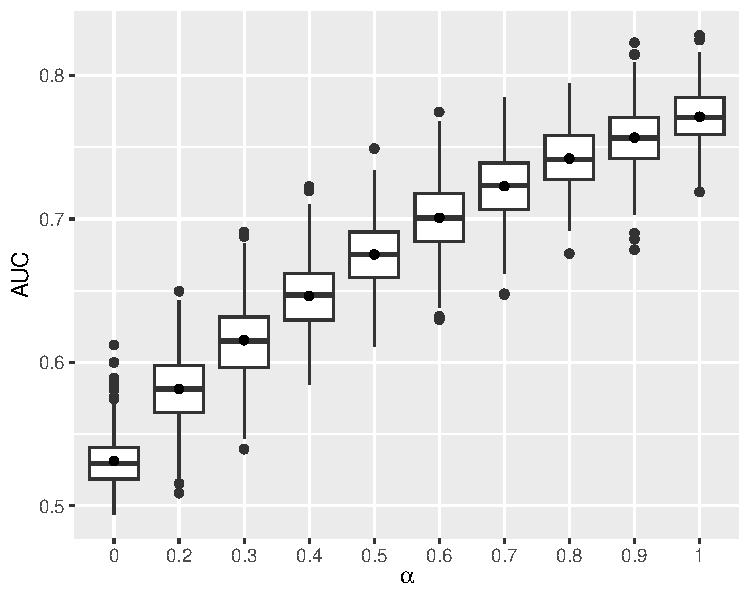
\includegraphics[width=5.5in]{../simFigs/alphaAUC.pdf}

\end{center}
%\begin{table}
%\caption{Coverage of nominal 95\% confidence intervals}
%\clearpage

\FloatBarrier
\subsection{Full Empirical 95\% Interval Coverage Results}
\FloatBarrier

The following tables give the empirical coverage of nominal 95\% intervals for \textsc{geepers} and mixture model principal effect estimates under varying data generating models. First we show results when $n=500$ per condition, and then when $n=1000$ per condition. \\

\begin{table}
  \caption{Empirical coverage of nominal 95\% Confidence intervals for \geepers and \pmm when $n=500$ per condition.}
  
\begin{tabular}[t]{lllrlllllll}
\toprule
\multicolumn{5}{c}{ } & \multicolumn{6}{c}{$n=500$} \\
\cmidrule(l{3pt}r{3pt}){6-11}
\multicolumn{5}{c}{ } & \multicolumn{2}{c}{$\alpha=0$} & \multicolumn{2}{c}{$\alpha=0.2$} & \multicolumn{2}{c}{$\alpha=0.5$} \\
\cmidrule(l{3pt}r{3pt}){6-7} \cmidrule(l{3pt}r{3pt}){8-9} \cmidrule(l{3pt}r{3pt}){10-11}
\makecell[l]{Residual\\Dist.} & \makecell[l]{$\bm{x}:Z$\\Int.?} & \makecell[l]{$\bm{x}:S_T$\\Int.?} & $\beta_1$ & \makecell[l]{Prin.\\Eff} & \textsc{geepers} & \textsc{pmm} & \textsc{geepers} & \textsc{pmm} & \textsc{geepers} & \textsc{pmm}\\
\midrule
 & No & No & 0.0 & $\tau^0$ & 1.00 & 1.00 & 0.98 & 0.98 & 0.97 & 0.96\\

 & No & No & 0.0 & $\tau^1$ & 1.00 & 1.00 & 0.97 & 0.97 & 0.97 & 0.95\\

 & Yes & No & 0.0 & $\tau^0$ & \rd{0.84} & \rd{0.70} & \rd{0.91} & \rd{0.74} & \rd{0.93} & \rd{0.81}\\

 & Yes & No & 0.0 & $\tau^1$ & \rd{0.85} & \rd{0.70} & \rd{0.91} & \rd{0.74} & \rd{0.93} & \rd{0.82}\\

 & No & Yes & 0.0 & $\tau^0$ & \rd{1.00} & \rd{1.00} & \rd{0.98} & \rd{0.99} & \rd{0.95} & \rd{0.95}\\

 & No & Yes & 0.0 & $\tau^1$ & \rd{1.00} & \rd{0.99} & \rd{0.98} & \rd{0.99} & \rd{0.95} & \rd{0.95}\\

 & Yes & Yes & 0.0 & $\tau^0$ & \rd{0.88} & \rd{0.76} & \rd{0.91} & \rd{0.77} & \rd{0.94} & \rd{0.83}\\

\multirow{-8}{*}{\raggedright\arraybackslash Normal} & Yes & Yes & 0.0 & $\tau^1$ & \rd{0.86} & \rd{0.74} & \rd{0.92} & \rd{0.76} & \rd{0.94} & \rd{0.82}\\
\cmidrule{1-11}
 & No & No & 0.0 & $\tau^0$ & 1.00 & \rd{0.15} & 0.96 & \rd{0.24} & 0.96 & \rd{0.50}\\

 & No & No & 0.0 & $\tau^1$ & 1.00 & \rd{0.16} & 0.97 & \rd{0.23} & 0.95 & \rd{0.49}\\

 & Yes & No & 0.0 & $\tau^0$ & \rd{0.85} & \rd{0.05} & \rd{0.83} & \rd{0.09} & \rd{0.95} & \rd{0.34}\\

 & Yes & No & 0.0 & $\tau^1$ & \rd{0.85} & \rd{0.06} & \rd{0.85} & \rd{0.09} & \rd{0.93} & \rd{0.33}\\

 & No & Yes & 0.0 & $\tau^0$ & \rd{1.00} & \rd{0.27} & \rd{0.99} & \rd{0.26} & \rd{0.95} & \rd{0.50}\\

 & No & Yes & 0.0 & $\tau^1$ & \rd{1.00} & \rd{0.28} & \rd{0.98} & \rd{0.26} & \rd{0.96} & \rd{0.52}\\

 & Yes & Yes & 0.0 & $\tau^0$ & \rd{0.83} & \rd{0.11} & \rd{0.86} & \rd{0.18} & \rd{0.92} & \rd{0.45}\\

\multirow{-8}{*}{\raggedright\arraybackslash Uniform} & Yes & Yes & 0.0 & $\tau^1$ & \rd{0.81} & \rd{0.11} & \rd{0.85} & \rd{0.17} & \rd{0.92} & \rd{0.45}\\
\cmidrule{1-11}
 & No & No & 0.3 & $\tau^0$ & 0.99 & 0.99 & 0.97 & 0.98 & 0.95 & 0.96\\

 & No & No & 0.3 & $\tau^1$ & 0.99 & 0.99 & 0.97 & 0.97 & 0.96 & 0.96\\

 & Yes & No & 0.3 & $\tau^0$ & \rd{0.88} & \rd{0.75} & \rd{0.88} & \rd{0.76} & \rd{0.94} & \rd{0.89}\\

 & Yes & No & 0.3 & $\tau^1$ & \rd{0.88} & \rd{0.74} & \rd{0.88} & \rd{0.74} & \rd{0.94} & \rd{0.89}\\

 & No & Yes & 0.3 & $\tau^0$ & \rd{0.99} & \rd{0.99} & \rd{0.97} & \rd{0.96} & \rd{0.96} & \rd{0.97}\\

 & No & Yes & 0.3 & $\tau^1$ & \rd{1.00} & \rd{1.00} & \rd{0.98} & \rd{0.97} & \rd{0.97} & \rd{0.96}\\

 & Yes & Yes & 0.3 & $\tau^0$ & \rd{0.90} & \rd{0.78} & \rd{0.90} & \rd{0.76} & \rd{0.93} & \rd{0.89}\\

\multirow{-8}{*}{\raggedright\arraybackslash Normal} & Yes & Yes & 0.3 & $\tau^1$ & \rd{0.90} & \rd{0.77} & \rd{0.90} & \rd{0.77} & \rd{0.94} & \rd{0.88}\\
\cmidrule{1-11}
 & No & No & 0.3 & $\tau^0$ & 0.99 & \rd{0.29} & 0.98 & \rd{0.39} & 0.95 & \rd{0.61}\\

 & No & No & 0.3 & $\tau^1$ & 0.99 & \rd{0.29} & 0.97 & \rd{0.40} & 0.95 & \rd{0.61}\\

 & Yes & No & 0.3 & $\tau^0$ & \rd{0.83} & \rd{0.12} & \rd{0.87} & \rd{0.21} & \rd{0.94} & \rd{0.48}\\

 & Yes & No & 0.3 & $\tau^1$ & \rd{0.83} & \rd{0.11} & \rd{0.87} & \rd{0.20} & \rd{0.93} & \rd{0.48}\\

 & No & Yes & 0.3 & $\tau^0$ & \rd{1.00} & \rd{0.47} & \rd{0.97} & \rd{0.49} & \rd{0.95} & \rd{0.60}\\

 & No & Yes & 0.3 & $\tau^1$ & \rd{1.00} & \rd{0.47} & \rd{0.98} & \rd{0.53} & \rd{0.96} & \rd{0.57}\\

 & Yes & Yes & 0.3 & $\tau^0$ & \rd{0.83} & \rd{0.16} & \rd{0.89} & \rd{0.21} & \rd{0.95} & \rd{0.52}\\

\multirow{-8}{*}{\raggedright\arraybackslash Uniform} & Yes & Yes & 0.3 & $\tau^1$ & \rd{0.83} & \rd{0.15} & \rd{0.88} & \rd{0.21} & \rd{0.94} & \rd{0.53}\\
\bottomrule
\end{tabular}

 \end{table}

 \begin{table}
  \caption{Empirical coverage of nominal 95\% Confidence intervals for \geepers and \pmm when $n=1000$ per condition.}
  
\begin{tabular}[t]{lllrlllllll}
\toprule
\multicolumn{5}{c}{ } & \multicolumn{6}{c}{$n=1000$} \\
\cmidrule(l{3pt}r{3pt}){6-11}
\multicolumn{5}{c}{ } & \multicolumn{2}{c}{$\alpha=0$} & \multicolumn{2}{c}{$\alpha=0.2$} & \multicolumn{2}{c}{$\alpha=0.5$} \\
\cmidrule(l{3pt}r{3pt}){6-7} \cmidrule(l{3pt}r{3pt}){8-9} \cmidrule(l{3pt}r{3pt}){10-11}
\makecell[l]{Residual\\Dist.} & \makecell[l]{X:Z\\Int.?} & \makecell[l]{X:S\\Int.?} & $\beta_1$ & \makecell[l]{Prin.\\Eff} & \geepers & \pmm & \geepers & \pmm & \geepers & \pmm\\
\midrule
 & No & No & 0.0 & $\tau^0$ & 1.00 & 1.00 & 0.97 & 0.96 & 0.94 & 0.94\\

 & No & No & 0.0 & $\tau^1$ & 1.00 & 1.00 & 0.96 & 0.96 & 0.95 & 0.95\\

 & Yes & No & 0.0 & $\tau^0$ & \rd{0.84} & \rd{0.48} & \rd{0.87} & \rd{0.51} & \rd{0.93} & \rd{0.75}\\

 & Yes & No & 0.0 & $\tau^1$ & \rd{0.85} & \rd{0.49} & \rd{0.87} & \rd{0.49} & \rd{0.93} & \rd{0.76}\\

 & No & Yes & 0.0 & $\tau^0$ & \rd{0.99} & \rd{1.00} & \rd{0.96} & \rd{0.97} & \rd{0.95} & \rd{0.95}\\

 & No & Yes & 0.0 & $\tau^1$ & \rd{0.99} & \rd{1.00} & \rd{0.96} & \rd{0.97} & \rd{0.95} & \rd{0.95}\\

 & Yes & Yes & 0.0 & $\tau^0$ & \rd{0.86} & \rd{0.53} & \rd{0.91} & \rd{0.55} & \rd{0.94} & \rd{0.80}\\

\multirow{-8}{*}{\raggedright\arraybackslash Normal} & Yes & Yes & 0.0 & $\tau^1$ & \rd{0.85} & \rd{0.52} & \rd{0.90} & \rd{0.55} & \rd{0.93} & \rd{0.78}\\
\cmidrule{1-11}
 & No & No & 0.0 & $\tau^0$ & 1.00 & \rd{0.00} & 0.97 & \rd{0.00} & 0.95 & \rd{0.21}\\

 & No & No & 0.0 & $\tau^1$ & 1.00 & \rd{0.00} & 0.97 & \rd{0.00} & 0.95 & \rd{0.22}\\

 & Yes & No & 0.0 & $\tau^0$ & \rd{0.87} & \rd{0.00} & \rd{0.88} & \rd{0.00} & \rd{0.92} & \rd{0.08}\\

 & Yes & No & 0.0 & $\tau^1$ & \rd{0.87} & \rd{0.00} & \rd{0.88} & \rd{0.00} & \rd{0.94} & \rd{0.08}\\

 & No & Yes & 0.0 & $\tau^0$ & \rd{1.00} & \rd{0.00} & \rd{0.98} & \rd{0.01} & \rd{0.94} & \rd{0.33}\\

 & No & Yes & 0.0 & $\tau^1$ & \rd{1.00} & \rd{0.00} & \rd{0.99} & \rd{0.01} & \rd{0.95} & \rd{0.33}\\

 & Yes & Yes & 0.0 & $\tau^0$ & \rd{0.80} & \rd{0.00} & \rd{0.87} & \rd{0.00} & \rd{0.91} & \rd{0.14}\\

\multirow{-8}{*}{\raggedright\arraybackslash Uniform} & Yes & Yes & 0.0 & $\tau^1$ & \rd{0.80} & \rd{0.00} & \rd{0.89} & \rd{0.00} & \rd{0.93} & \rd{0.14}\\
\cmidrule{1-11}
 & No & No & 0.3 & $\tau^0$ & 1.00 & 1.00 & 0.96 & 0.97 & 0.94 & 0.94\\

 & No & No & 0.3 & $\tau^1$ & 1.00 & 0.99 & 0.97 & 0.97 & 0.95 & 0.96\\

 & Yes & No & 0.3 & $\tau^0$ & \rd{0.87} & \rd{0.55} & \rd{0.89} & \rd{0.60} & \rd{0.94} & \rd{0.80}\\

 & Yes & No & 0.3 & $\tau^1$ & \rd{0.87} & \rd{0.55} & \rd{0.90} & \rd{0.60} & \rd{0.93} & \rd{0.79}\\

 & No & Yes & 0.3 & $\tau^0$ & \rd{1.00} & \rd{1.00} & \rd{0.97} & \rd{0.96} & \rd{0.95} & \rd{0.97}\\

 & No & Yes & 0.3 & $\tau^1$ & \rd{1.00} & \rd{1.00} & \rd{0.97} & \rd{0.97} & \rd{0.94} & \rd{0.96}\\

 & Yes & Yes & 0.3 & $\tau^0$ & \rd{0.86} & \rd{0.55} & \rd{0.91} & \rd{0.62} & \rd{0.95} & \rd{0.83}\\

\multirow{-8}{*}{\raggedright\arraybackslash Normal} & Yes & Yes & 0.3 & $\tau^1$ & \rd{0.85} & \rd{0.54} & \rd{0.91} & \rd{0.62} & \rd{0.91} & \rd{0.81}\\
\cmidrule{1-11}
 & No & No & 0.3 & $\tau^0$ & 0.99 & \rd{0.00} & 0.95 & \rd{0.01} & 0.96 & \rd{0.31}\\

 & No & No & 0.3 & $\tau^1$ & 1.00 & \rd{0.00} & 0.95 & \rd{0.01} & 0.96 & \rd{0.30}\\

 & Yes & No & 0.3 & $\tau^0$ & \rd{0.88} & \rd{0.00} & \rd{0.91} & \rd{0.00} & \rd{0.91} & \rd{0.17}\\

 & Yes & No & 0.3 & $\tau^1$ & \rd{0.88} & \rd{0.00} & \rd{0.90} & \rd{0.00} & \rd{0.92} & \rd{0.17}\\

 & No & Yes & 0.3 & $\tau^0$ & \rd{1.00} & \rd{0.02} & \rd{0.96} & \rd{0.07} & \rd{0.97} & \rd{0.41}\\

 & No & Yes & 0.3 & $\tau^1$ & \rd{1.00} & \rd{0.02} & \rd{0.95} & \rd{0.07} & \rd{0.97} & \rd{0.40}\\

 & Yes & Yes & 0.3 & $\tau^0$ & \rd{0.87} & \rd{0.00} & \rd{0.89} & \rd{0.03} & \rd{0.95} & \rd{0.22}\\

\multirow{-8}{*}{\raggedright\arraybackslash Uniform} & Yes & Yes & 0.3 & $\tau^1$ & \rd{0.86} & \rd{0.00} & \rd{0.87} & \rd{0.03} & \rd{0.92} & \rd{0.21}\\
\bottomrule
\end{tabular}

 \end{table}


 

%\clearpage
\FloatBarrier
\subsection{Full RMSE Results}
\FloatBarrier

The following table gives the root mean squared error (RMSE), $\left\{\sum_b (\hat{\tau}-\tau)^2/500\right\}^{1/2}$, for \textsc{geepers}, mixture model, and principal score weighting principal effect estimates under varying data generating models.\\

\begin{table}
  \caption{Empirical RMSE  for \geepers, \pmm, and \psw when $n=500$ per condition.}
  
\begin{tabular}[t]{llllrrrrrr}
\toprule
\multicolumn{4}{c}{ } & \multicolumn{6}{c}{$n=500$} \\
\cmidrule(l{3pt}r{3pt}){5-10}
\multicolumn{4}{c}{ } & \multicolumn{3}{c}{$\alpha=0.2$} & \multicolumn{3}{c}{$\alpha=0.5$} \\
\cmidrule(l{3pt}r{3pt}){5-7} \cmidrule(l{3pt}r{3pt}){8-10}
\makecell[l]{Residual\\Dist.} & \makecell[l]{$\bm{x}:Z$\\Int.?} & \makecell[l]{$\bm{x}:S_T$\\Int.?} & Parameter & \textsc{geepers} & \textsc{pmm} & \textsc{psw} & \textsc{geepers} & \textsc{pmm} & \textsc{psw}\\
\midrule
 & No & No & $\tau^0$ & 0.56 & 0.17 & 0.09 & 0.17 & 0.15 & 0.11\\

 & No & No & $\tau^1$ & 0.57 & 0.17 & 0.08 & 0.17 & 0.15 & 0.12\\

 & Yes & No & $\tau^0$ & 0.94 & 0.29 & 0.09 & 0.23 & 0.23 & 0.12\\

 & Yes & No & $\tau^1$ & 0.94 & 0.30 & 0.09 & 0.23 & 0.23 & 0.13\\

 & No & Yes & $\tau^0$ & 0.48 & 0.17 & 0.08 & 0.18 & 0.16 & 0.11\\

 & No & Yes & $\tau^1$ & 0.46 & 0.16 & 0.08 & 0.18 & 0.15 & 0.12\\

 & Yes & Yes & $\tau^0$ & 0.98 & 0.29 & 0.09 & 0.23 & 0.23 & 0.12\\

\multirow{-8}{*}{\raggedright\arraybackslash Normal} & Yes & Yes & $\tau^1$ & 0.99 & 0.29 & 0.09 & 0.23 & 0.23 & 0.12\\
\cmidrule{1-10}
 & No & No & $\tau^0$ & 0.42 & 0.55 & 0.09 & 0.18 & 0.42 & 0.11\\

 & No & No & $\tau^1$ & 0.42 & 0.54 & 0.08 & 0.18 & 0.42 & 0.12\\

 & Yes & No & $\tau^0$ & 1.58 & 0.58 & 0.09 & 0.22 & 0.46 & 0.12\\

 & Yes & No & $\tau^1$ & 1.60 & 0.57 & 0.08 & 0.22 & 0.46 & 0.12\\

 & No & Yes & $\tau^0$ & 0.41 & 0.53 & 0.09 & 0.19 & 0.41 & 0.11\\

 & No & Yes & $\tau^1$ & 0.41 & 0.54 & 0.08 & 0.19 & 0.41 & 0.12\\

 & Yes & Yes & $\tau^0$ & 2.70 & 0.55 & 0.09 & 0.23 & 0.44 & 0.12\\

\multirow{-8}{*}{\raggedright\arraybackslash Uniform} & Yes & Yes & $\tau^1$ & 2.29 & 0.57 & 0.09 & 0.24 & 0.44 & 0.13\\
\bottomrule
\end{tabular}

 \end{table}


 \begin{table}
  \caption{Empirical RMSE  for \geepers, \pmm, and \psw when $n=1000$ per condition.}
  
\begin{tabular}[t]{lllrlll}
\toprule
\multicolumn{5}{c}{ } & \multicolumn{6}{c}{$n=1000$} \\
\cmidrule(l{3pt}r{3pt}){6-11}
\multicolumn{5}{c}{ } & \multicolumn{3}{c}{$\alpha=0.2$} & \multicolumn{3}{c}{$\alpha=0.5$} \\
\cmidrule(l{3pt}r{3pt}){6-8} \cmidrule(l{3pt}r{3pt}){9-11}
\makecell[l]{Residual\\Dist.} & \makecell[l]{$\bm{x}:Z$\\Int.?} & \makecell[l]{$\bm{x}:S_T$\\Int.?} & $\beta_1$ & \makecell[l]{Prin.\\Eff} & NA & NA\\
\midrule
 & No & No & 0.0 & $\tau^0$ & 0.28614523, 0.15955541, 0.06634178 & 0.1334332, 0.1118913, 0.2301330\\

 & No & No & 0.0 & $\tau^1$ & 0.28698999, 0.16003274, 0.06642983 & 0.1312804, 0.1101555, 0.2263442\\

 & Yes & No & 0.0 & $\tau^0$ & 0.63273196, 0.33191436, 0.06793985 & 0.1602354, 0.1542353, 0.2280050\\

 & Yes & No & 0.0 & $\tau^1$ & 0.63687828, 0.33633998, 0.07082269 & 0.1660086, 0.1621297, 0.2340535\\

 & No & Yes & 0.0 & $\tau^0$ & 0.29800383, 0.15846149, 0.06277431 & 0.1337284, 0.1084597, 0.2297158\\

 & No & Yes & 0.0 & $\tau^1$ & 0.29743087, 0.15779350, 0.06785113 & 0.1343788, 0.1088816, 0.2293977\\

 & Yes & Yes & 0.0 & $\tau^0$ & 0.65217667, 0.32705412, 0.06552952 & 0.1597539, 0.1563865, 0.2315080\\

\multirow{-8}{*}{\raggedright\arraybackslash Normal} & Yes & Yes & 0.0 & $\tau^1$ & 0.66944417, 0.33455905, 0.07120576 & 0.1730754, 0.1594959, 0.2311189\\
\cmidrule{1-7}
 & No & No & 0.0 & $\tau^0$ & 0.30553664, 0.60640609, 0.06835612 & 0.1286616, 0.3204181, 0.2300569\\

 & No & No & 0.0 & $\tau^1$ & 0.30740028, 0.60569824, 0.06483881 & 0.1302221, 0.3264583, 0.2292238\\

 & Yes & No & 0.0 & $\tau^0$ & 0.61409087, 0.59784266, 0.07504119 & 0.1635624, 0.3625994, 0.2305085\\

 & Yes & No & 0.0 & $\tau^1$ & 0.61363329, 0.59955143, 0.06869204 & 0.1673316, 0.3597955, 0.2371051\\

 & No & Yes & 0.0 & $\tau^0$ & 0.26886669, 0.59409192, 0.06710054 & 0.1206525, 0.2890499, 0.2303636\\

 & No & Yes & 0.0 & $\tau^1$ & 0.26397806, 0.59693309, 0.06601589 & 0.1213490, 0.2878535, 0.2355593\\

 & Yes & Yes & 0.0 & $\tau^0$ & 0.59569881, 0.60088276, 0.06370024 & 0.1566310, 0.3441396, 0.2306057\\

\multirow{-8}{*}{\raggedright\arraybackslash Uniform} & Yes & Yes & 0.0 & $\tau^1$ & 0.60498441, 0.60193854, 0.07007712 & 0.1656667, 0.3366524, 0.2327784\\
\cmidrule{1-7}
 & No & No & 0.3 & $\tau^0$ & 0.2827230, 0.1737796, 0.1939610 & 0.1334332, 0.1118913, 0.2301330\\

 & No & No & 0.3 & $\tau^1$ & 0.2830708, 0.1712405, 0.1901653 & 0.1312804, 0.1101555, 0.2263442\\

 & Yes & No & 0.3 & $\tau^0$ & 0.6542264, 0.3440573, 0.1966910 & 0.1602354, 0.1542353, 0.2280050\\

 & Yes & No & 0.3 & $\tau^1$ & 0.6611211, 0.3508378, 0.1933766 & 0.1660086, 0.1621297, 0.2340535\\

 & No & Yes & 0.3 & $\tau^0$ & 0.2802360, 0.1810313, 0.1929841 & 0.1337284, 0.1084597, 0.2297158\\

 & No & Yes & 0.3 & $\tau^1$ & 0.2837333, 0.1831605, 0.1979786 & 0.1343788, 0.1088816, 0.2293977\\

 & Yes & Yes & 0.3 & $\tau^0$ & 0.6512733, 0.3317055, 0.1964653 & 0.1597539, 0.1563865, 0.2315080\\

\multirow{-8}{*}{\raggedright\arraybackslash Normal} & Yes & Yes & 0.3 & $\tau^1$ & 0.6570717, 0.3399707, 0.1932301 & 0.1730754, 0.1594959, 0.2311189\\
\cmidrule{1-7}
 & No & No & 0.3 & $\tau^0$ & 0.3539324, 0.5749586, 0.1917318 & 0.1286616, 0.3204181, 0.2300569\\

 & No & No & 0.3 & $\tau^1$ & 0.3555457, 0.5805273, 0.1929551 & 0.1302221, 0.3264583, 0.2292238\\

 & Yes & No & 0.3 & $\tau^0$ & 0.5915788, 0.6068832, 0.2007860 & 0.1635624, 0.3625994, 0.2305085\\

 & Yes & No & 0.3 & $\tau^1$ & 0.6047826, 0.6099683, 0.1931586 & 0.1673316, 0.3597955, 0.2371051\\

 & No & Yes & 0.3 & $\tau^0$ & 0.2763328, 0.5714127, 0.1958715 & 0.1206525, 0.2890499, 0.2303636\\

 & No & Yes & 0.3 & $\tau^1$ & 0.2704888, 0.5695698, 0.1926049 & 0.1213490, 0.2878535, 0.2355593\\

 & Yes & Yes & 0.3 & $\tau^0$ & 0.6718339, 0.5789302, 0.1904290 & 0.1566310, 0.3441396, 0.2306057\\

\multirow{-8}{*}{\raggedright\arraybackslash Uniform} & Yes & Yes & 0.3 & $\tau^1$ & 0.6902849, 0.5810495, 0.1982476 & 0.1656667, 0.3366524, 0.2327784\\
\bottomrule
\end{tabular}

 \end{table}

%\end{table}
%\clearpage


\FloatBarrier
\section{Additional Results from the OPT Study}
\FloatBarrier
\singlespacing
\FloatBarrier
\subsection{Summary Statistics}
\FloatBarrier
The following table gives summary statistics for covariates and post-treatment outcomes in two of the conditions from the empirical study.\\

\begin{table}

\caption{\label{tab:optTab1}Descriptive statistics---mean and standard deviation or count and percent---for study variables in the full OPT dataset and in the analysis sample (i.e., complete cases)}
\centering
\begin{tabular}[t]{lllll}
\toprule
\multicolumn{1}{c}{ } & \multicolumn{2}{c}{Full Data} & \multicolumn{2}{c}{Complete Cases} \\
\cmidrule(l{3pt}r{3pt}){2-3} \cmidrule(l{3pt}r{3pt}){4-5}
  & Control & Treatment & Control & Treatment\\
\midrule
n & 410 & 413 & 326 & 314\\
Fibrinogen & 21.3 (14.9) & 20.2 (13.3) & 21.5 (15.4) & 20 (13.1)\\
Endotoxin & 1.8 (1.1) & 1.8 (1.1) & 1.8 (1.1) & 1.8 (1.1)\\
\% Sites Bleeding & 67.3 (21.1) & 43.9 (20.4) & 67.6 (21.3) & 43.5 (20.3)\\
Trt. Completed: No & - & 14 (3.4\%) & - & 4 (1.3\%)\\
\addlinespace
Trt. Completed: Und & - & 196 (47.5\%) & - & 153 (48.7\%)\\
Trt. Completed: Yes & - & 185 (44.8\%) & - & 157 (50\%)\\
\bottomrule
\end{tabular}
\end{table}


%\clearpage
\FloatBarrier
\section{Additional Results from the Bottoming-Out Study}
\singlespacing
The following table gives summary statistics for covariates and post-treatment outcomes in two of the conditions from the empirical study.\\

\FloatBarrier
\subsection{Summary Statistics}
\FloatBarrier

The following table gives summary statistics for covariates and post-treatment outcomes in two of the conditions from the empirical study.\\
\small
% latex table generated in R 4.2.2 by xtable 1.8-4 package
% Mon Nov  6 17:52:58 2023
\begin{sidewaystable}[ht]
\centering
\begin{tabular}{llllllll}
  \hline
  &   & ASSISTments & BAU & Dragon & FH2T & Miss. \% & Imp. Err. (PFC) \\ 
  \hline
n &  &  402 &  385 &  369 &  791 &      &  \\ 
  Modality & In-Person &  260 (64.7)  &  238 (61.8)  &  241 (65.3)  &  529 (66.9)  &  0.0 & 0 \\ 
   & Remote &  142 (35.3)  &  147 (38.2)  &  128 (34.7)  &  262 (33.1)  &      &  \\ 
  Gender & Female &  206 (51.2)  &  193 (50.1)  &  178 (48.2)  &  376 (47.5)  &  0.0 & 0 \\ 
   & Male &  196 (48.8)  &  192 (49.9)  &  191 (51.8)  &  415 (52.5)  &      &  \\ 
  Race/Ethnicity & White &  213 (53.0)  &  192 (49.9)  &  182 (49.5)  &  409 (51.7)  &  0.1 & 0.28 \\ 
   & Hispanic/Latino &   56 (13.9)  &   51 (13.2)  &   67 (18.2)  &  120 (15.2)  &      &  \\ 
   & Asian &   98 (24.4)  &  106 (27.5)  &   89 (24.2)  &  198 (25.0)  &      &  \\ 
   & Other &   35 ( 8.7)  &   36 ( 9.4)  &   30 ( 8.2)  &   64 ( 8.1)  &      &  \\ 
  Grade 5 Perf. Lev. & Beginning Learner &   12 ( 3.3)  &    8 ( 2.4)  &   14 ( 4.5)  &   23 ( 3.3)  & 12.4 & 0.01 \\ 
   & Developing Learner &   64 (17.8)  &   62 (18.3)  &   53 (16.9)  &  124 (17.9)  &      &  \\ 
   & Distinguished Learner &  158 (43.9)  &  152 (45.0)  &  141 (44.9)  &  306 (44.2)  &      &  \\ 
   & Proficient Learner &  126 (35.0)  &  116 (34.3)  &  106 (33.8)  &  240 (34.6)  &      &  \\ 
  Pretest-Procedural &  & 1.70 (0.92) & 1.55 (1.01) & 1.64 (0.96) & 1.57 (0.98) &  5.0 & 0.42 \\ 
  Pretest-Flexibility &  & 1.47 (0.93) & 1.43 (0.93) & 1.51 (0.91) & 1.49 (0.92) &  5.0 & 0.4 \\ 
  Has EIP &  &  31 ( 7.7)  &  27 ( 7.0)  &  31 ( 8.4)  &  56 ( 7.1)  &  0.0 & 0 \\ 
  ESOL &  &  31 ( 7.7)  &  36 ( 9.4)  &  45 (12.2)  &  75 ( 9.5)  &  0.0 & 0 \\ 
  Gifted &  &  72 (17.9)  &  69 (17.9)  &  53 (14.4)  & 129 (16.3)  &  0.0 & 0 \\ 
  Has IEP &  &  38 ( 9.5)  &  40 (10.4)  &  41 (11.1)  &  60 ( 7.6)  &  0.0 & 0 \\ 
  IST &  &  25 ( 6.9)  &  27 ( 7.8)  &  23 ( 7.3)  &  58 ( 8.3)  & 11.6 & 0.06 \\ 
  SECTION504 &  &  14 ( 3.9)  &  10 ( 2.9)  &   7 ( 2.2)  &  14 ( 2.0)  & 11.6 & 0.03 \\ 
  SST &  &  11 ( 3.0)  &  12 ( 3.5)  &  13 ( 4.1)  &  31 ( 4.4)  & 11.6 & 0.03 \\ 
  fullYear5 &  & 337 (93.4)  & 321 (93.3)  & 298 (94.3)  & 659 (94.1)  & 11.6 & 0.06 \\ 
  fullYear6 &  & 368 (96.3)  & 353 (95.7)  & 328 (93.4)  & 728 (95.9)  &  4.4 & 0.04 \\ 
  noUnexcused5 &  & 112 (31.0)  &  98 (28.5)  &  93 (29.4)  & 200 (28.6)  & 11.6 & 0 \\ 
   \hline
Bottom-Outer &  & 191 (47.5)  &   0 ( 0.0)  &   0 ( 0.0)  &   0 ( 0.0)  &  0.0 &  \\ 
   \hline
\end{tabular}
\caption{Counts and percentages for categorical study variables, by randomized condition. Imputation error is the proportion falsly classified, as estimated using by missForest using out-of-bag observations. All variables were measured at baseline, with the exception of "Bottom-Outer," the principal stratification variable.} 
\label{table:tab1fac}
\end{sidewaystable}

%\clearpage

\small
% latex table generated in R 4.2.2 by xtable 1.8-4 package
% Mon Nov  6 15:43:04 2023
\begin{sidewaystable}[ht]
\centering
\begin{tabular}{rlllll}
  \hline
 & ASSISTments & BAU & Dragon & Miss. \% & Imp. Err. (NRMSE) \\ 
  \hline
n &    402 &    385 &    369 &    791 &  \\ 
  Grade 5 Stand. Test & 575.32 (61.16) & 578.82 (59.86) & 574.24 (63.32) & 576.20 (60.99) & 784.69 \\ 
  log(Days Abs. 5th+1) &   1.49 (0.77) &   1.55 (0.78) &   1.48 (0.76) &   1.54 (0.81) & 0.29 \\ 
  log(Days Unexc. 5th+1) &   0.87 (0.72) &   0.93 (0.73) &   0.86 (0.69) &   0.93 (0.74) & 0.12 \\ 
  log(Days Abs. 6th+1) &   1.32 (0.73) &   1.29 (0.74) &   1.26 (0.71) &   1.33 (0.76) & 0.22 \\ 
  log(Days Unexc. 6th+1) &   0.80 (0.66) &   0.80 (0.64) &   0.72 (0.62) &   0.82 (0.69) & 0.2 \\ 
  Pretest &   4.89 (2.70) &   4.73 (2.70) &   4.99 (2.60) &   4.80 (2.69) & 1.02 \\ 
  Pretest-\# Completed &   9.36 (2.33) &   9.27 (2.45) &   9.18 (2.68) &   9.47 (2.13) & 0 \\ 
  log(Pretest ToT) &   6.41 (0.74) &   6.40 (0.83) &   6.45 (0.71) &   6.44 (0.76) & 0.37 \\ 
  Math Anxiety &  13.93 (5.66) &  13.72 (5.98) &  12.94 (5.71) &  13.62 (5.91) & 23.22 \\ 
  Math Self-Eff &  17.19 (4.95) &  17.44 (4.78) &  18.10 (4.55) &  17.63 (4.77) & 15.06 \\ 
  Perceptual Sens. &   7.50 (2.91) &   7.71 (2.94) &   7.44 (3.16) &   7.46 (3.00) & 0.54 \\ 
  Perc. Sens. Pt 2E &   1.37 (1.26) &   1.38 (1.24) &   1.41 (1.32) &   1.37 (1.28) & 0.47 \\ 
  Perc. Sens. Pt 2NE &   1.15 (1.08) &   1.18 (1.12) &   1.17 (1.18) &   1.07 (1.09) & 0.47 \\ 
  Perc. Sens. \#Comp. &  14.81 (3.93) &  14.54 (4.39) &  14.38 (4.62) &  14.91 (3.75) & 0 \\ 
  log(PS Resp. Time) &   5.74 (0.82) &   5.78 (0.88) &   5.76 (0.84) &   5.72 (0.84) & 0.4 \\ 
   \hline
\# Bottom-Out &  22.62 (28.65) &   1.27 (8.98) &   4.72 (9.48) &   6.54 (14.72) &  \\ 
  Posttest &   4.52 (2.88) &   4.26 (2.79) &   4.75 (2.87) &   4.54 (2.95) &  \\ 
   \hline
\end{tabular}
\caption{Means and standard deviations for numeric study variables, by randomized condition. Imputation error is the normalized root mean squared error (NRMSE), as estimated using by missForest using out-of-bag observations. All variables were measured at baseline, with the exception of "\# Bottom-Out" (the number of bottom-out hints requested) and Posttest.} 
\label{table:tab1num}
\end{sidewaystable}

\FloatBarrier
\subsection{Regression Results}
\FloatBarrier

Regression estimates from three principal score logit models and three outcome regressions, based on the "All Covariates" principal score model, for \textsc{geepers} estimates. Standard errors shown are nominal regression errors, not sandwich corrected. Fixed-effect estimates for school (PS-models) or classroom (outcome models) are omitted.

\small
%
  \providecommand{\huxb}[2]{\arrayrulecolor[RGB]{#1}\global\arrayrulewidth=#2pt}
  \providecommand{\huxvb}[2]{\color[RGB]{#1}\vrule width #2pt}
  \providecommand{\huxtpad}[1]{\rule{0pt}{#1}}
  \providecommand{\huxbpad}[1]{\rule[-#1]{0pt}{#1}}

\begin{table}[ht]
\begin{centerbox}
\begin{threeparttable}
 \setlength{\tabcolsep}{0pt}
\begin{tabular}{l l l l l}


\hhline{>{\huxb{0, 0, 0}{0.8}}->{\huxb{0, 0, 0}{0.8}}->{\huxb{0, 0, 0}{0.8}}->{\huxb{0, 0, 0}{0.8}}->{\huxb{0, 0, 0}{0.8}}-}
\arrayrulecolor{black}

\multicolumn{1}{!{\huxvb{0, 0, 0}{0}}c!{\huxvb{0, 0, 0}{0}}}{\huxtpad{6pt + 1em}\centering \hspace{6pt}  \hspace{6pt}\huxbpad{6pt}} &
\multicolumn{1}{c!{\huxvb{0, 0, 0}{0}}}{\huxtpad{6pt + 1em}\centering \hspace{6pt} psModel \hspace{6pt}\huxbpad{6pt}} &
\multicolumn{1}{c!{\huxvb{0, 0, 0}{0}}}{\huxtpad{6pt + 1em}\centering \hspace{6pt} BAU \hspace{6pt}\huxbpad{6pt}} &
\multicolumn{1}{c!{\huxvb{0, 0, 0}{0}}}{\huxtpad{6pt + 1em}\centering \hspace{6pt} FH2T \hspace{6pt}\huxbpad{6pt}} &
\multicolumn{1}{c!{\huxvb{0, 0, 0}{0}}}{\huxtpad{6pt + 1em}\centering \hspace{6pt} DragonBox \hspace{6pt}\huxbpad{6pt}} \tabularnewline[-0.5pt]


\hhline{>{\huxb{255, 255, 255}{0.4}}->{\huxb{0, 0, 0}{0.4}}->{\huxb{0, 0, 0}{0.4}}->{\huxb{0, 0, 0}{0.4}}->{\huxb{0, 0, 0}{0.4}}-}
\arrayrulecolor{black}

\multicolumn{1}{!{\huxvb{0, 0, 0}{0}}l!{\huxvb{0, 0, 0}{0}}}{\huxtpad{6pt + 1em}\raggedright \hspace{6pt} (Intercept) \hspace{6pt}\huxbpad{6pt}} &
\multicolumn{1}{r!{\huxvb{0, 0, 0}{0}}}{\huxtpad{6pt + 1em}\raggedleft \hspace{6pt} -2.143\hphantom{0}\hphantom{0}\hphantom{0}\hphantom{0} \hspace{6pt}\huxbpad{6pt}} &
\multicolumn{1}{r!{\huxvb{0, 0, 0}{0}}}{\huxtpad{6pt + 1em}\raggedleft \hspace{6pt} 1.732\hphantom{0}\hphantom{0}\hphantom{0} \hspace{6pt}\huxbpad{6pt}} &
\multicolumn{1}{r!{\huxvb{0, 0, 0}{0}}}{\huxtpad{6pt + 1em}\raggedleft \hspace{6pt} 2.834 *** \hspace{6pt}\huxbpad{6pt}} &
\multicolumn{1}{r!{\huxvb{0, 0, 0}{0}}}{\huxtpad{6pt + 1em}\raggedleft \hspace{6pt} 2.510 **\hphantom{0} \hspace{6pt}\huxbpad{6pt}} \tabularnewline[-0.5pt]


\hhline{}
\arrayrulecolor{black}

\multicolumn{1}{!{\huxvb{0, 0, 0}{0}}l!{\huxvb{0, 0, 0}{0}}}{\huxtpad{6pt + 1em}\raggedright \hspace{6pt}  \hspace{6pt}\huxbpad{6pt}} &
\multicolumn{1}{r!{\huxvb{0, 0, 0}{0}}}{\huxtpad{6pt + 1em}\raggedleft \hspace{6pt} (1.257)\hphantom{0}\hphantom{0}\hphantom{0} \hspace{6pt}\huxbpad{6pt}} &
\multicolumn{1}{r!{\huxvb{0, 0, 0}{0}}}{\huxtpad{6pt + 1em}\raggedleft \hspace{6pt} (0.916)\hphantom{0}\hphantom{0} \hspace{6pt}\huxbpad{6pt}} &
\multicolumn{1}{r!{\huxvb{0, 0, 0}{0}}}{\huxtpad{6pt + 1em}\raggedleft \hspace{6pt} (0.718)\hphantom{0}\hphantom{0}\hphantom{0} \hspace{6pt}\huxbpad{6pt}} &
\multicolumn{1}{r!{\huxvb{0, 0, 0}{0}}}{\huxtpad{6pt + 1em}\raggedleft \hspace{6pt} (0.919)\hphantom{0}\hphantom{0}\hphantom{0} \hspace{6pt}\huxbpad{6pt}} \tabularnewline[-0.5pt]


\hhline{}
\arrayrulecolor{black}

\multicolumn{1}{!{\huxvb{0, 0, 0}{0}}l!{\huxvb{0, 0, 0}{0}}}{\huxtpad{6pt + 1em}\raggedright \hspace{6pt} Scale.Score5 \hspace{6pt}\huxbpad{6pt}} &
\multicolumn{1}{r!{\huxvb{0, 0, 0}{0}}}{\huxtpad{6pt + 1em}\raggedleft \hspace{6pt} -0.594 **\hphantom{0} \hspace{6pt}\huxbpad{6pt}} &
\multicolumn{1}{r!{\huxvb{0, 0, 0}{0}}}{\huxtpad{6pt + 1em}\raggedleft \hspace{6pt} 0.207\hphantom{0}\hphantom{0}\hphantom{0} \hspace{6pt}\huxbpad{6pt}} &
\multicolumn{1}{r!{\huxvb{0, 0, 0}{0}}}{\huxtpad{6pt + 1em}\raggedleft \hspace{6pt} 0.453 *** \hspace{6pt}\huxbpad{6pt}} &
\multicolumn{1}{r!{\huxvb{0, 0, 0}{0}}}{\huxtpad{6pt + 1em}\raggedleft \hspace{6pt} 0.049\hphantom{0}\hphantom{0}\hphantom{0}\hphantom{0} \hspace{6pt}\huxbpad{6pt}} \tabularnewline[-0.5pt]


\hhline{}
\arrayrulecolor{black}

\multicolumn{1}{!{\huxvb{0, 0, 0}{0}}l!{\huxvb{0, 0, 0}{0}}}{\huxtpad{6pt + 1em}\raggedright \hspace{6pt}  \hspace{6pt}\huxbpad{6pt}} &
\multicolumn{1}{r!{\huxvb{0, 0, 0}{0}}}{\huxtpad{6pt + 1em}\raggedleft \hspace{6pt} (0.188)\hphantom{0}\hphantom{0}\hphantom{0} \hspace{6pt}\huxbpad{6pt}} &
\multicolumn{1}{r!{\huxvb{0, 0, 0}{0}}}{\huxtpad{6pt + 1em}\raggedleft \hspace{6pt} (0.126)\hphantom{0}\hphantom{0} \hspace{6pt}\huxbpad{6pt}} &
\multicolumn{1}{r!{\huxvb{0, 0, 0}{0}}}{\huxtpad{6pt + 1em}\raggedleft \hspace{6pt} (0.104)\hphantom{0}\hphantom{0}\hphantom{0} \hspace{6pt}\huxbpad{6pt}} &
\multicolumn{1}{r!{\huxvb{0, 0, 0}{0}}}{\huxtpad{6pt + 1em}\raggedleft \hspace{6pt} (0.132)\hphantom{0}\hphantom{0}\hphantom{0} \hspace{6pt}\huxbpad{6pt}} \tabularnewline[-0.5pt]


\hhline{}
\arrayrulecolor{black}

\multicolumn{1}{!{\huxvb{0, 0, 0}{0}}l!{\huxvb{0, 0, 0}{0}}}{\huxtpad{6pt + 1em}\raggedright \hspace{6pt} ESOL1 \hspace{6pt}\huxbpad{6pt}} &
\multicolumn{1}{r!{\huxvb{0, 0, 0}{0}}}{\huxtpad{6pt + 1em}\raggedleft \hspace{6pt} -0.825\hphantom{0}\hphantom{0}\hphantom{0}\hphantom{0} \hspace{6pt}\huxbpad{6pt}} &
\multicolumn{1}{r!{\huxvb{0, 0, 0}{0}}}{\huxtpad{6pt + 1em}\raggedleft \hspace{6pt} 0.091\hphantom{0}\hphantom{0}\hphantom{0} \hspace{6pt}\huxbpad{6pt}} &
\multicolumn{1}{r!{\huxvb{0, 0, 0}{0}}}{\huxtpad{6pt + 1em}\raggedleft \hspace{6pt} -0.459\hphantom{0}\hphantom{0}\hphantom{0}\hphantom{0} \hspace{6pt}\huxbpad{6pt}} &
\multicolumn{1}{r!{\huxvb{0, 0, 0}{0}}}{\huxtpad{6pt + 1em}\raggedleft \hspace{6pt} -0.493\hphantom{0}\hphantom{0}\hphantom{0}\hphantom{0} \hspace{6pt}\huxbpad{6pt}} \tabularnewline[-0.5pt]


\hhline{}
\arrayrulecolor{black}

\multicolumn{1}{!{\huxvb{0, 0, 0}{0}}l!{\huxvb{0, 0, 0}{0}}}{\huxtpad{6pt + 1em}\raggedright \hspace{6pt}  \hspace{6pt}\huxbpad{6pt}} &
\multicolumn{1}{r!{\huxvb{0, 0, 0}{0}}}{\huxtpad{6pt + 1em}\raggedleft \hspace{6pt} (0.642)\hphantom{0}\hphantom{0}\hphantom{0} \hspace{6pt}\huxbpad{6pt}} &
\multicolumn{1}{r!{\huxvb{0, 0, 0}{0}}}{\huxtpad{6pt + 1em}\raggedleft \hspace{6pt} (0.364)\hphantom{0}\hphantom{0} \hspace{6pt}\huxbpad{6pt}} &
\multicolumn{1}{r!{\huxvb{0, 0, 0}{0}}}{\huxtpad{6pt + 1em}\raggedleft \hspace{6pt} (0.268)\hphantom{0}\hphantom{0}\hphantom{0} \hspace{6pt}\huxbpad{6pt}} &
\multicolumn{1}{r!{\huxvb{0, 0, 0}{0}}}{\huxtpad{6pt + 1em}\raggedleft \hspace{6pt} (0.351)\hphantom{0}\hphantom{0}\hphantom{0} \hspace{6pt}\huxbpad{6pt}} \tabularnewline[-0.5pt]


\hhline{}
\arrayrulecolor{black}

\multicolumn{1}{!{\huxvb{0, 0, 0}{0}}l!{\huxvb{0, 0, 0}{0}}}{\huxtpad{6pt + 1em}\raggedright \hspace{6pt} IEP1 \hspace{6pt}\huxbpad{6pt}} &
\multicolumn{1}{r!{\huxvb{0, 0, 0}{0}}}{\huxtpad{6pt + 1em}\raggedleft \hspace{6pt} -1.335 **\hphantom{0} \hspace{6pt}\huxbpad{6pt}} &
\multicolumn{1}{r!{\huxvb{0, 0, 0}{0}}}{\huxtpad{6pt + 1em}\raggedleft \hspace{6pt} 0.148\hphantom{0}\hphantom{0}\hphantom{0} \hspace{6pt}\huxbpad{6pt}} &
\multicolumn{1}{r!{\huxvb{0, 0, 0}{0}}}{\huxtpad{6pt + 1em}\raggedleft \hspace{6pt} 0.234\hphantom{0}\hphantom{0}\hphantom{0}\hphantom{0} \hspace{6pt}\huxbpad{6pt}} &
\multicolumn{1}{r!{\huxvb{0, 0, 0}{0}}}{\huxtpad{6pt + 1em}\raggedleft \hspace{6pt} 0.096\hphantom{0}\hphantom{0}\hphantom{0}\hphantom{0} \hspace{6pt}\huxbpad{6pt}} \tabularnewline[-0.5pt]


\hhline{}
\arrayrulecolor{black}

\multicolumn{1}{!{\huxvb{0, 0, 0}{0}}l!{\huxvb{0, 0, 0}{0}}}{\huxtpad{6pt + 1em}\raggedright \hspace{6pt}  \hspace{6pt}\huxbpad{6pt}} &
\multicolumn{1}{r!{\huxvb{0, 0, 0}{0}}}{\huxtpad{6pt + 1em}\raggedleft \hspace{6pt} (0.463)\hphantom{0}\hphantom{0}\hphantom{0} \hspace{6pt}\huxbpad{6pt}} &
\multicolumn{1}{r!{\huxvb{0, 0, 0}{0}}}{\huxtpad{6pt + 1em}\raggedleft \hspace{6pt} (0.288)\hphantom{0}\hphantom{0} \hspace{6pt}\huxbpad{6pt}} &
\multicolumn{1}{r!{\huxvb{0, 0, 0}{0}}}{\huxtpad{6pt + 1em}\raggedleft \hspace{6pt} (0.255)\hphantom{0}\hphantom{0}\hphantom{0} \hspace{6pt}\huxbpad{6pt}} &
\multicolumn{1}{r!{\huxvb{0, 0, 0}{0}}}{\huxtpad{6pt + 1em}\raggedleft \hspace{6pt} (0.277)\hphantom{0}\hphantom{0}\hphantom{0} \hspace{6pt}\huxbpad{6pt}} \tabularnewline[-0.5pt]


\hhline{}
\arrayrulecolor{black}

\multicolumn{1}{!{\huxvb{0, 0, 0}{0}}l!{\huxvb{0, 0, 0}{0}}}{\huxtpad{6pt + 1em}\raggedright \hspace{6pt} pre.total\_time\_on\_tasks \hspace{6pt}\huxbpad{6pt}} &
\multicolumn{1}{r!{\huxvb{0, 0, 0}{0}}}{\huxtpad{6pt + 1em}\raggedleft \hspace{6pt} -0.447 **\hphantom{0} \hspace{6pt}\huxbpad{6pt}} &
\multicolumn{1}{r!{\huxvb{0, 0, 0}{0}}}{\huxtpad{6pt + 1em}\raggedleft \hspace{6pt} -0.131\hphantom{0}\hphantom{0}\hphantom{0} \hspace{6pt}\huxbpad{6pt}} &
\multicolumn{1}{r!{\huxvb{0, 0, 0}{0}}}{\huxtpad{6pt + 1em}\raggedleft \hspace{6pt} 0.078\hphantom{0}\hphantom{0}\hphantom{0}\hphantom{0} \hspace{6pt}\huxbpad{6pt}} &
\multicolumn{1}{r!{\huxvb{0, 0, 0}{0}}}{\huxtpad{6pt + 1em}\raggedleft \hspace{6pt} -0.003\hphantom{0}\hphantom{0}\hphantom{0}\hphantom{0} \hspace{6pt}\huxbpad{6pt}} \tabularnewline[-0.5pt]


\hhline{}
\arrayrulecolor{black}

\multicolumn{1}{!{\huxvb{0, 0, 0}{0}}l!{\huxvb{0, 0, 0}{0}}}{\huxtpad{6pt + 1em}\raggedright \hspace{6pt}  \hspace{6pt}\huxbpad{6pt}} &
\multicolumn{1}{r!{\huxvb{0, 0, 0}{0}}}{\huxtpad{6pt + 1em}\raggedleft \hspace{6pt} (0.152)\hphantom{0}\hphantom{0}\hphantom{0} \hspace{6pt}\huxbpad{6pt}} &
\multicolumn{1}{r!{\huxvb{0, 0, 0}{0}}}{\huxtpad{6pt + 1em}\raggedleft \hspace{6pt} (0.091)\hphantom{0}\hphantom{0} \hspace{6pt}\huxbpad{6pt}} &
\multicolumn{1}{r!{\huxvb{0, 0, 0}{0}}}{\huxtpad{6pt + 1em}\raggedleft \hspace{6pt} (0.073)\hphantom{0}\hphantom{0}\hphantom{0} \hspace{6pt}\huxbpad{6pt}} &
\multicolumn{1}{r!{\huxvb{0, 0, 0}{0}}}{\huxtpad{6pt + 1em}\raggedleft \hspace{6pt} (0.096)\hphantom{0}\hphantom{0}\hphantom{0} \hspace{6pt}\huxbpad{6pt}} \tabularnewline[-0.5pt]


\hhline{}
\arrayrulecolor{black}

\multicolumn{1}{!{\huxvb{0, 0, 0}{0}}l!{\huxvb{0, 0, 0}{0}}}{\huxtpad{6pt + 1em}\raggedright \hspace{6pt} pre\_MSE\_total\_score \hspace{6pt}\huxbpad{6pt}} &
\multicolumn{1}{r!{\huxvb{0, 0, 0}{0}}}{\huxtpad{6pt + 1em}\raggedleft \hspace{6pt} -0.179\hphantom{0}\hphantom{0}\hphantom{0}\hphantom{0} \hspace{6pt}\huxbpad{6pt}} &
\multicolumn{1}{r!{\huxvb{0, 0, 0}{0}}}{\huxtpad{6pt + 1em}\raggedleft \hspace{6pt} 0.201 *\hphantom{0} \hspace{6pt}\huxbpad{6pt}} &
\multicolumn{1}{r!{\huxvb{0, 0, 0}{0}}}{\huxtpad{6pt + 1em}\raggedleft \hspace{6pt} 0.120\hphantom{0}\hphantom{0}\hphantom{0}\hphantom{0} \hspace{6pt}\huxbpad{6pt}} &
\multicolumn{1}{r!{\huxvb{0, 0, 0}{0}}}{\huxtpad{6pt + 1em}\raggedleft \hspace{6pt} 0.350 *** \hspace{6pt}\huxbpad{6pt}} \tabularnewline[-0.5pt]


\hhline{}
\arrayrulecolor{black}

\multicolumn{1}{!{\huxvb{0, 0, 0}{0}}l!{\huxvb{0, 0, 0}{0}}}{\huxtpad{6pt + 1em}\raggedright \hspace{6pt}  \hspace{6pt}\huxbpad{6pt}} &
\multicolumn{1}{r!{\huxvb{0, 0, 0}{0}}}{\huxtpad{6pt + 1em}\raggedleft \hspace{6pt} (0.130)\hphantom{0}\hphantom{0}\hphantom{0} \hspace{6pt}\huxbpad{6pt}} &
\multicolumn{1}{r!{\huxvb{0, 0, 0}{0}}}{\huxtpad{6pt + 1em}\raggedleft \hspace{6pt} (0.082)\hphantom{0}\hphantom{0} \hspace{6pt}\huxbpad{6pt}} &
\multicolumn{1}{r!{\huxvb{0, 0, 0}{0}}}{\huxtpad{6pt + 1em}\raggedleft \hspace{6pt} (0.068)\hphantom{0}\hphantom{0}\hphantom{0} \hspace{6pt}\huxbpad{6pt}} &
\multicolumn{1}{r!{\huxvb{0, 0, 0}{0}}}{\huxtpad{6pt + 1em}\raggedleft \hspace{6pt} (0.084)\hphantom{0}\hphantom{0}\hphantom{0} \hspace{6pt}\huxbpad{6pt}} \tabularnewline[-0.5pt]


\hhline{}
\arrayrulecolor{black}

\multicolumn{1}{!{\huxvb{0, 0, 0}{0}}l!{\huxvb{0, 0, 0}{0}}}{\huxtpad{6pt + 1em}\raggedright \hspace{6pt} fullYear5TRUE \hspace{6pt}\huxbpad{6pt}} &
\multicolumn{1}{r!{\huxvb{0, 0, 0}{0}}}{\huxtpad{6pt + 1em}\raggedleft \hspace{6pt} 1.405 *\hphantom{0}\hphantom{0} \hspace{6pt}\huxbpad{6pt}} &
\multicolumn{1}{r!{\huxvb{0, 0, 0}{0}}}{\huxtpad{6pt + 1em}\raggedleft \hspace{6pt} -0.129\hphantom{0}\hphantom{0}\hphantom{0} \hspace{6pt}\huxbpad{6pt}} &
\multicolumn{1}{r!{\huxvb{0, 0, 0}{0}}}{\huxtpad{6pt + 1em}\raggedleft \hspace{6pt} -0.099\hphantom{0}\hphantom{0}\hphantom{0}\hphantom{0} \hspace{6pt}\huxbpad{6pt}} &
\multicolumn{1}{r!{\huxvb{0, 0, 0}{0}}}{\huxtpad{6pt + 1em}\raggedleft \hspace{6pt} 0.062\hphantom{0}\hphantom{0}\hphantom{0}\hphantom{0} \hspace{6pt}\huxbpad{6pt}} \tabularnewline[-0.5pt]


\hhline{}
\arrayrulecolor{black}

\multicolumn{1}{!{\huxvb{0, 0, 0}{0}}l!{\huxvb{0, 0, 0}{0}}}{\huxtpad{6pt + 1em}\raggedright \hspace{6pt}  \hspace{6pt}\huxbpad{6pt}} &
\multicolumn{1}{r!{\huxvb{0, 0, 0}{0}}}{\huxtpad{6pt + 1em}\raggedleft \hspace{6pt} (0.585)\hphantom{0}\hphantom{0}\hphantom{0} \hspace{6pt}\huxbpad{6pt}} &
\multicolumn{1}{r!{\huxvb{0, 0, 0}{0}}}{\huxtpad{6pt + 1em}\raggedleft \hspace{6pt} (0.328)\hphantom{0}\hphantom{0} \hspace{6pt}\huxbpad{6pt}} &
\multicolumn{1}{r!{\huxvb{0, 0, 0}{0}}}{\huxtpad{6pt + 1em}\raggedleft \hspace{6pt} (0.286)\hphantom{0}\hphantom{0}\hphantom{0} \hspace{6pt}\huxbpad{6pt}} &
\multicolumn{1}{r!{\huxvb{0, 0, 0}{0}}}{\huxtpad{6pt + 1em}\raggedleft \hspace{6pt} (0.341)\hphantom{0}\hphantom{0}\hphantom{0} \hspace{6pt}\huxbpad{6pt}} \tabularnewline[-0.5pt]


\hhline{}
\arrayrulecolor{black}

\multicolumn{1}{!{\huxvb{0, 0, 0}{0}}l!{\huxvb{0, 0, 0}{0}}}{\huxtpad{6pt + 1em}\raggedright \hspace{6pt} pre\_MA\_total\_scoreNATRUE \hspace{6pt}\huxbpad{6pt}} &
\multicolumn{1}{r!{\huxvb{0, 0, 0}{0}}}{\huxtpad{6pt + 1em}\raggedleft \hspace{6pt} -3.205 *** \hspace{6pt}\huxbpad{6pt}} &
\multicolumn{1}{r!{\huxvb{0, 0, 0}{0}}}{\huxtpad{6pt + 1em}\raggedleft \hspace{6pt} \hphantom{0}\hphantom{0}\hphantom{0}\hphantom{0}\hphantom{0}\hphantom{0}\hphantom{0} \hspace{6pt}\huxbpad{6pt}} &
\multicolumn{1}{r!{\huxvb{0, 0, 0}{0}}}{\huxtpad{6pt + 1em}\raggedleft \hspace{6pt} \hphantom{0}\hphantom{0}\hphantom{0}\hphantom{0}\hphantom{0}\hphantom{0}\hphantom{0}\hphantom{0} \hspace{6pt}\huxbpad{6pt}} &
\multicolumn{1}{r!{\huxvb{0, 0, 0}{0}}}{\huxtpad{6pt + 1em}\raggedleft \hspace{6pt} \hphantom{0}\hphantom{0}\hphantom{0}\hphantom{0}\hphantom{0}\hphantom{0}\hphantom{0}\hphantom{0} \hspace{6pt}\huxbpad{6pt}} \tabularnewline[-0.5pt]


\hhline{}
\arrayrulecolor{black}

\multicolumn{1}{!{\huxvb{0, 0, 0}{0}}l!{\huxvb{0, 0, 0}{0}}}{\huxtpad{6pt + 1em}\raggedright \hspace{6pt}  \hspace{6pt}\huxbpad{6pt}} &
\multicolumn{1}{r!{\huxvb{0, 0, 0}{0}}}{\huxtpad{6pt + 1em}\raggedleft \hspace{6pt} (0.706)\hphantom{0}\hphantom{0}\hphantom{0} \hspace{6pt}\huxbpad{6pt}} &
\multicolumn{1}{r!{\huxvb{0, 0, 0}{0}}}{\huxtpad{6pt + 1em}\raggedleft \hspace{6pt} \hphantom{0}\hphantom{0}\hphantom{0}\hphantom{0}\hphantom{0}\hphantom{0}\hphantom{0} \hspace{6pt}\huxbpad{6pt}} &
\multicolumn{1}{r!{\huxvb{0, 0, 0}{0}}}{\huxtpad{6pt + 1em}\raggedleft \hspace{6pt} \hphantom{0}\hphantom{0}\hphantom{0}\hphantom{0}\hphantom{0}\hphantom{0}\hphantom{0}\hphantom{0} \hspace{6pt}\huxbpad{6pt}} &
\multicolumn{1}{r!{\huxvb{0, 0, 0}{0}}}{\huxtpad{6pt + 1em}\raggedleft \hspace{6pt} \hphantom{0}\hphantom{0}\hphantom{0}\hphantom{0}\hphantom{0}\hphantom{0}\hphantom{0}\hphantom{0} \hspace{6pt}\huxbpad{6pt}} \tabularnewline[-0.5pt]


\hhline{}
\arrayrulecolor{black}

\multicolumn{1}{!{\huxvb{0, 0, 0}{0}}l!{\huxvb{0, 0, 0}{0}}}{\huxtpad{6pt + 1em}\raggedright \hspace{6pt} GenderM \hspace{6pt}\huxbpad{6pt}} &
\multicolumn{1}{r!{\huxvb{0, 0, 0}{0}}}{\huxtpad{6pt + 1em}\raggedleft \hspace{6pt} 0.169\hphantom{0}\hphantom{0}\hphantom{0}\hphantom{0} \hspace{6pt}\huxbpad{6pt}} &
\multicolumn{1}{r!{\huxvb{0, 0, 0}{0}}}{\huxtpad{6pt + 1em}\raggedleft \hspace{6pt} -0.186\hphantom{0}\hphantom{0}\hphantom{0} \hspace{6pt}\huxbpad{6pt}} &
\multicolumn{1}{r!{\huxvb{0, 0, 0}{0}}}{\huxtpad{6pt + 1em}\raggedleft \hspace{6pt} -0.337 **\hphantom{0} \hspace{6pt}\huxbpad{6pt}} &
\multicolumn{1}{r!{\huxvb{0, 0, 0}{0}}}{\huxtpad{6pt + 1em}\raggedleft \hspace{6pt} -0.267\hphantom{0}\hphantom{0}\hphantom{0}\hphantom{0} \hspace{6pt}\huxbpad{6pt}} \tabularnewline[-0.5pt]


\hhline{}
\arrayrulecolor{black}

\multicolumn{1}{!{\huxvb{0, 0, 0}{0}}l!{\huxvb{0, 0, 0}{0}}}{\huxtpad{6pt + 1em}\raggedright \hspace{6pt}  \hspace{6pt}\huxbpad{6pt}} &
\multicolumn{1}{r!{\huxvb{0, 0, 0}{0}}}{\huxtpad{6pt + 1em}\raggedleft \hspace{6pt} (0.253)\hphantom{0}\hphantom{0}\hphantom{0} \hspace{6pt}\huxbpad{6pt}} &
\multicolumn{1}{r!{\huxvb{0, 0, 0}{0}}}{\huxtpad{6pt + 1em}\raggedleft \hspace{6pt} (0.155)\hphantom{0}\hphantom{0} \hspace{6pt}\huxbpad{6pt}} &
\multicolumn{1}{r!{\huxvb{0, 0, 0}{0}}}{\huxtpad{6pt + 1em}\raggedleft \hspace{6pt} (0.125)\hphantom{0}\hphantom{0}\hphantom{0} \hspace{6pt}\huxbpad{6pt}} &
\multicolumn{1}{r!{\huxvb{0, 0, 0}{0}}}{\huxtpad{6pt + 1em}\raggedleft \hspace{6pt} (0.155)\hphantom{0}\hphantom{0}\hphantom{0} \hspace{6pt}\huxbpad{6pt}} \tabularnewline[-0.5pt]


\hhline{}
\arrayrulecolor{black}

\multicolumn{1}{!{\huxvb{0, 0, 0}{0}}l!{\huxvb{0, 0, 0}{0}}}{\huxtpad{6pt + 1em}\raggedright \hspace{6pt} raceEthHispanic/Latino \hspace{6pt}\huxbpad{6pt}} &
\multicolumn{1}{r!{\huxvb{0, 0, 0}{0}}}{\huxtpad{6pt + 1em}\raggedleft \hspace{6pt} -0.561\hphantom{0}\hphantom{0}\hphantom{0}\hphantom{0} \hspace{6pt}\huxbpad{6pt}} &
\multicolumn{1}{r!{\huxvb{0, 0, 0}{0}}}{\huxtpad{6pt + 1em}\raggedleft \hspace{6pt} 0.275\hphantom{0}\hphantom{0}\hphantom{0} \hspace{6pt}\huxbpad{6pt}} &
\multicolumn{1}{r!{\huxvb{0, 0, 0}{0}}}{\huxtpad{6pt + 1em}\raggedleft \hspace{6pt} 0.327\hphantom{0}\hphantom{0}\hphantom{0}\hphantom{0} \hspace{6pt}\huxbpad{6pt}} &
\multicolumn{1}{r!{\huxvb{0, 0, 0}{0}}}{\huxtpad{6pt + 1em}\raggedleft \hspace{6pt} 0.225\hphantom{0}\hphantom{0}\hphantom{0}\hphantom{0} \hspace{6pt}\huxbpad{6pt}} \tabularnewline[-0.5pt]


\hhline{}
\arrayrulecolor{black}

\multicolumn{1}{!{\huxvb{0, 0, 0}{0}}l!{\huxvb{0, 0, 0}{0}}}{\huxtpad{6pt + 1em}\raggedright \hspace{6pt}  \hspace{6pt}\huxbpad{6pt}} &
\multicolumn{1}{r!{\huxvb{0, 0, 0}{0}}}{\huxtpad{6pt + 1em}\raggedleft \hspace{6pt} (0.460)\hphantom{0}\hphantom{0}\hphantom{0} \hspace{6pt}\huxbpad{6pt}} &
\multicolumn{1}{r!{\huxvb{0, 0, 0}{0}}}{\huxtpad{6pt + 1em}\raggedleft \hspace{6pt} (0.290)\hphantom{0}\hphantom{0} \hspace{6pt}\huxbpad{6pt}} &
\multicolumn{1}{r!{\huxvb{0, 0, 0}{0}}}{\huxtpad{6pt + 1em}\raggedleft \hspace{6pt} (0.213)\hphantom{0}\hphantom{0}\hphantom{0} \hspace{6pt}\huxbpad{6pt}} &
\multicolumn{1}{r!{\huxvb{0, 0, 0}{0}}}{\huxtpad{6pt + 1em}\raggedleft \hspace{6pt} (0.283)\hphantom{0}\hphantom{0}\hphantom{0} \hspace{6pt}\huxbpad{6pt}} \tabularnewline[-0.5pt]


\hhline{}
\arrayrulecolor{black}

\multicolumn{1}{!{\huxvb{0, 0, 0}{0}}l!{\huxvb{0, 0, 0}{0}}}{\huxtpad{6pt + 1em}\raggedright \hspace{6pt} raceEthAsian \hspace{6pt}\huxbpad{6pt}} &
\multicolumn{1}{r!{\huxvb{0, 0, 0}{0}}}{\huxtpad{6pt + 1em}\raggedleft \hspace{6pt} -0.431\hphantom{0}\hphantom{0}\hphantom{0}\hphantom{0} \hspace{6pt}\huxbpad{6pt}} &
\multicolumn{1}{r!{\huxvb{0, 0, 0}{0}}}{\huxtpad{6pt + 1em}\raggedleft \hspace{6pt} 0.662 *\hphantom{0} \hspace{6pt}\huxbpad{6pt}} &
\multicolumn{1}{r!{\huxvb{0, 0, 0}{0}}}{\huxtpad{6pt + 1em}\raggedleft \hspace{6pt} 0.619 **\hphantom{0} \hspace{6pt}\huxbpad{6pt}} &
\multicolumn{1}{r!{\huxvb{0, 0, 0}{0}}}{\huxtpad{6pt + 1em}\raggedleft \hspace{6pt} 0.823 **\hphantom{0} \hspace{6pt}\huxbpad{6pt}} \tabularnewline[-0.5pt]


\hhline{}
\arrayrulecolor{black}

\multicolumn{1}{!{\huxvb{0, 0, 0}{0}}l!{\huxvb{0, 0, 0}{0}}}{\huxtpad{6pt + 1em}\raggedright \hspace{6pt}  \hspace{6pt}\huxbpad{6pt}} &
\multicolumn{1}{r!{\huxvb{0, 0, 0}{0}}}{\huxtpad{6pt + 1em}\raggedleft \hspace{6pt} (0.416)\hphantom{0}\hphantom{0}\hphantom{0} \hspace{6pt}\huxbpad{6pt}} &
\multicolumn{1}{r!{\huxvb{0, 0, 0}{0}}}{\huxtpad{6pt + 1em}\raggedleft \hspace{6pt} (0.279)\hphantom{0}\hphantom{0} \hspace{6pt}\huxbpad{6pt}} &
\multicolumn{1}{r!{\huxvb{0, 0, 0}{0}}}{\huxtpad{6pt + 1em}\raggedleft \hspace{6pt} (0.225)\hphantom{0}\hphantom{0}\hphantom{0} \hspace{6pt}\huxbpad{6pt}} &
\multicolumn{1}{r!{\huxvb{0, 0, 0}{0}}}{\huxtpad{6pt + 1em}\raggedleft \hspace{6pt} (0.298)\hphantom{0}\hphantom{0}\hphantom{0} \hspace{6pt}\huxbpad{6pt}} \tabularnewline[-0.5pt]


\hhline{}
\arrayrulecolor{black}

\multicolumn{1}{!{\huxvb{0, 0, 0}{0}}l!{\huxvb{0, 0, 0}{0}}}{\huxtpad{6pt + 1em}\raggedright \hspace{6pt} raceEthOther \hspace{6pt}\huxbpad{6pt}} &
\multicolumn{1}{r!{\huxvb{0, 0, 0}{0}}}{\huxtpad{6pt + 1em}\raggedleft \hspace{6pt} -0.131\hphantom{0}\hphantom{0}\hphantom{0}\hphantom{0} \hspace{6pt}\huxbpad{6pt}} &
\multicolumn{1}{r!{\huxvb{0, 0, 0}{0}}}{\huxtpad{6pt + 1em}\raggedleft \hspace{6pt} 0.455\hphantom{0}\hphantom{0}\hphantom{0} \hspace{6pt}\huxbpad{6pt}} &
\multicolumn{1}{r!{\huxvb{0, 0, 0}{0}}}{\huxtpad{6pt + 1em}\raggedleft \hspace{6pt} 0.208\hphantom{0}\hphantom{0}\hphantom{0}\hphantom{0} \hspace{6pt}\huxbpad{6pt}} &
\multicolumn{1}{r!{\huxvb{0, 0, 0}{0}}}{\huxtpad{6pt + 1em}\raggedleft \hspace{6pt} 0.095\hphantom{0}\hphantom{0}\hphantom{0}\hphantom{0} \hspace{6pt}\huxbpad{6pt}} \tabularnewline[-0.5pt]


\hhline{}
\arrayrulecolor{black}

\multicolumn{1}{!{\huxvb{0, 0, 0}{0}}l!{\huxvb{0, 0, 0}{0}}}{\huxtpad{6pt + 1em}\raggedright \hspace{6pt}  \hspace{6pt}\huxbpad{6pt}} &
\multicolumn{1}{r!{\huxvb{0, 0, 0}{0}}}{\huxtpad{6pt + 1em}\raggedleft \hspace{6pt} (0.492)\hphantom{0}\hphantom{0}\hphantom{0} \hspace{6pt}\huxbpad{6pt}} &
\multicolumn{1}{r!{\huxvb{0, 0, 0}{0}}}{\huxtpad{6pt + 1em}\raggedleft \hspace{6pt} (0.292)\hphantom{0}\hphantom{0} \hspace{6pt}\huxbpad{6pt}} &
\multicolumn{1}{r!{\huxvb{0, 0, 0}{0}}}{\huxtpad{6pt + 1em}\raggedleft \hspace{6pt} (0.231)\hphantom{0}\hphantom{0}\hphantom{0} \hspace{6pt}\huxbpad{6pt}} &
\multicolumn{1}{r!{\huxvb{0, 0, 0}{0}}}{\huxtpad{6pt + 1em}\raggedleft \hspace{6pt} (0.300)\hphantom{0}\hphantom{0}\hphantom{0} \hspace{6pt}\huxbpad{6pt}} \tabularnewline[-0.5pt]


\hhline{}
\arrayrulecolor{black}

\multicolumn{1}{!{\huxvb{0, 0, 0}{0}}l!{\huxvb{0, 0, 0}{0}}}{\huxtpad{6pt + 1em}\raggedright \hspace{6pt} GIFTED1 \hspace{6pt}\huxbpad{6pt}} &
\multicolumn{1}{r!{\huxvb{0, 0, 0}{0}}}{\huxtpad{6pt + 1em}\raggedleft \hspace{6pt} -0.240\hphantom{0}\hphantom{0}\hphantom{0}\hphantom{0} \hspace{6pt}\huxbpad{6pt}} &
\multicolumn{1}{r!{\huxvb{0, 0, 0}{0}}}{\huxtpad{6pt + 1em}\raggedleft \hspace{6pt} 0.659 ** \hspace{6pt}\huxbpad{6pt}} &
\multicolumn{1}{r!{\huxvb{0, 0, 0}{0}}}{\huxtpad{6pt + 1em}\raggedleft \hspace{6pt} 0.429 *\hphantom{0}\hphantom{0} \hspace{6pt}\huxbpad{6pt}} &
\multicolumn{1}{r!{\huxvb{0, 0, 0}{0}}}{\huxtpad{6pt + 1em}\raggedleft \hspace{6pt} 0.336\hphantom{0}\hphantom{0}\hphantom{0}\hphantom{0} \hspace{6pt}\huxbpad{6pt}} \tabularnewline[-0.5pt]


\hhline{}
\arrayrulecolor{black}

\multicolumn{1}{!{\huxvb{0, 0, 0}{0}}l!{\huxvb{0, 0, 0}{0}}}{\huxtpad{6pt + 1em}\raggedright \hspace{6pt}  \hspace{6pt}\huxbpad{6pt}} &
\multicolumn{1}{r!{\huxvb{0, 0, 0}{0}}}{\huxtpad{6pt + 1em}\raggedleft \hspace{6pt} (0.371)\hphantom{0}\hphantom{0}\hphantom{0} \hspace{6pt}\huxbpad{6pt}} &
\multicolumn{1}{r!{\huxvb{0, 0, 0}{0}}}{\huxtpad{6pt + 1em}\raggedleft \hspace{6pt} (0.243)\hphantom{0}\hphantom{0} \hspace{6pt}\huxbpad{6pt}} &
\multicolumn{1}{r!{\huxvb{0, 0, 0}{0}}}{\huxtpad{6pt + 1em}\raggedleft \hspace{6pt} (0.192)\hphantom{0}\hphantom{0}\hphantom{0} \hspace{6pt}\huxbpad{6pt}} &
\multicolumn{1}{r!{\huxvb{0, 0, 0}{0}}}{\huxtpad{6pt + 1em}\raggedleft \hspace{6pt} (0.260)\hphantom{0}\hphantom{0}\hphantom{0} \hspace{6pt}\huxbpad{6pt}} \tabularnewline[-0.5pt]


\hhline{}
\arrayrulecolor{black}

\multicolumn{1}{!{\huxvb{0, 0, 0}{0}}l!{\huxvb{0, 0, 0}{0}}}{\huxtpad{6pt + 1em}\raggedright \hspace{6pt} poly(pre\_PS\_tasks\_total\_score, 2, raw = TRUE)1 \hspace{6pt}\huxbpad{6pt}} &
\multicolumn{1}{r!{\huxvb{0, 0, 0}{0}}}{\huxtpad{6pt + 1em}\raggedleft \hspace{6pt} 0.006\hphantom{0}\hphantom{0}\hphantom{0}\hphantom{0} \hspace{6pt}\huxbpad{6pt}} &
\multicolumn{1}{r!{\huxvb{0, 0, 0}{0}}}{\huxtpad{6pt + 1em}\raggedleft \hspace{6pt} \hphantom{0}\hphantom{0}\hphantom{0}\hphantom{0}\hphantom{0}\hphantom{0}\hphantom{0} \hspace{6pt}\huxbpad{6pt}} &
\multicolumn{1}{r!{\huxvb{0, 0, 0}{0}}}{\huxtpad{6pt + 1em}\raggedleft \hspace{6pt} \hphantom{0}\hphantom{0}\hphantom{0}\hphantom{0}\hphantom{0}\hphantom{0}\hphantom{0}\hphantom{0} \hspace{6pt}\huxbpad{6pt}} &
\multicolumn{1}{r!{\huxvb{0, 0, 0}{0}}}{\huxtpad{6pt + 1em}\raggedleft \hspace{6pt} \hphantom{0}\hphantom{0}\hphantom{0}\hphantom{0}\hphantom{0}\hphantom{0}\hphantom{0}\hphantom{0} \hspace{6pt}\huxbpad{6pt}} \tabularnewline[-0.5pt]


\hhline{}
\arrayrulecolor{black}

\multicolumn{1}{!{\huxvb{0, 0, 0}{0}}l!{\huxvb{0, 0, 0}{0}}}{\huxtpad{6pt + 1em}\raggedright \hspace{6pt}  \hspace{6pt}\huxbpad{6pt}} &
\multicolumn{1}{r!{\huxvb{0, 0, 0}{0}}}{\huxtpad{6pt + 1em}\raggedleft \hspace{6pt} (0.191)\hphantom{0}\hphantom{0}\hphantom{0} \hspace{6pt}\huxbpad{6pt}} &
\multicolumn{1}{r!{\huxvb{0, 0, 0}{0}}}{\huxtpad{6pt + 1em}\raggedleft \hspace{6pt} \hphantom{0}\hphantom{0}\hphantom{0}\hphantom{0}\hphantom{0}\hphantom{0}\hphantom{0} \hspace{6pt}\huxbpad{6pt}} &
\multicolumn{1}{r!{\huxvb{0, 0, 0}{0}}}{\huxtpad{6pt + 1em}\raggedleft \hspace{6pt} \hphantom{0}\hphantom{0}\hphantom{0}\hphantom{0}\hphantom{0}\hphantom{0}\hphantom{0}\hphantom{0} \hspace{6pt}\huxbpad{6pt}} &
\multicolumn{1}{r!{\huxvb{0, 0, 0}{0}}}{\huxtpad{6pt + 1em}\raggedleft \hspace{6pt} \hphantom{0}\hphantom{0}\hphantom{0}\hphantom{0}\hphantom{0}\hphantom{0}\hphantom{0}\hphantom{0} \hspace{6pt}\huxbpad{6pt}} \tabularnewline[-0.5pt]


\hhline{}
\arrayrulecolor{black}

\multicolumn{1}{!{\huxvb{0, 0, 0}{0}}l!{\huxvb{0, 0, 0}{0}}}{\huxtpad{6pt + 1em}\raggedright \hspace{6pt} poly(pre\_PS\_tasks\_total\_score, 2, raw = TRUE)2 \hspace{6pt}\huxbpad{6pt}} &
\multicolumn{1}{r!{\huxvb{0, 0, 0}{0}}}{\huxtpad{6pt + 1em}\raggedleft \hspace{6pt} -0.407 **\hphantom{0} \hspace{6pt}\huxbpad{6pt}} &
\multicolumn{1}{r!{\huxvb{0, 0, 0}{0}}}{\huxtpad{6pt + 1em}\raggedleft \hspace{6pt} \hphantom{0}\hphantom{0}\hphantom{0}\hphantom{0}\hphantom{0}\hphantom{0}\hphantom{0} \hspace{6pt}\huxbpad{6pt}} &
\multicolumn{1}{r!{\huxvb{0, 0, 0}{0}}}{\huxtpad{6pt + 1em}\raggedleft \hspace{6pt} \hphantom{0}\hphantom{0}\hphantom{0}\hphantom{0}\hphantom{0}\hphantom{0}\hphantom{0}\hphantom{0} \hspace{6pt}\huxbpad{6pt}} &
\multicolumn{1}{r!{\huxvb{0, 0, 0}{0}}}{\huxtpad{6pt + 1em}\raggedleft \hspace{6pt} \hphantom{0}\hphantom{0}\hphantom{0}\hphantom{0}\hphantom{0}\hphantom{0}\hphantom{0}\hphantom{0} \hspace{6pt}\huxbpad{6pt}} \tabularnewline[-0.5pt]


\hhline{}
\arrayrulecolor{black}

\multicolumn{1}{!{\huxvb{0, 0, 0}{0}}l!{\huxvb{0, 0, 0}{0}}}{\huxtpad{6pt + 1em}\raggedright \hspace{6pt}  \hspace{6pt}\huxbpad{6pt}} &
\multicolumn{1}{r!{\huxvb{0, 0, 0}{0}}}{\huxtpad{6pt + 1em}\raggedleft \hspace{6pt} (0.133)\hphantom{0}\hphantom{0}\hphantom{0} \hspace{6pt}\huxbpad{6pt}} &
\multicolumn{1}{r!{\huxvb{0, 0, 0}{0}}}{\huxtpad{6pt + 1em}\raggedleft \hspace{6pt} \hphantom{0}\hphantom{0}\hphantom{0}\hphantom{0}\hphantom{0}\hphantom{0}\hphantom{0} \hspace{6pt}\huxbpad{6pt}} &
\multicolumn{1}{r!{\huxvb{0, 0, 0}{0}}}{\huxtpad{6pt + 1em}\raggedleft \hspace{6pt} \hphantom{0}\hphantom{0}\hphantom{0}\hphantom{0}\hphantom{0}\hphantom{0}\hphantom{0}\hphantom{0} \hspace{6pt}\huxbpad{6pt}} &
\multicolumn{1}{r!{\huxvb{0, 0, 0}{0}}}{\huxtpad{6pt + 1em}\raggedleft \hspace{6pt} \hphantom{0}\hphantom{0}\hphantom{0}\hphantom{0}\hphantom{0}\hphantom{0}\hphantom{0}\hphantom{0} \hspace{6pt}\huxbpad{6pt}} \tabularnewline[-0.5pt]


\hhline{}
\arrayrulecolor{black}

\multicolumn{1}{!{\huxvb{0, 0, 0}{0}}l!{\huxvb{0, 0, 0}{0}}}{\huxtpad{6pt + 1em}\raggedright \hspace{6pt} Z \hspace{6pt}\huxbpad{6pt}} &
\multicolumn{1}{r!{\huxvb{0, 0, 0}{0}}}{\huxtpad{6pt + 1em}\raggedleft \hspace{6pt} \hphantom{0}\hphantom{0}\hphantom{0}\hphantom{0}\hphantom{0}\hphantom{0}\hphantom{0}\hphantom{0} \hspace{6pt}\huxbpad{6pt}} &
\multicolumn{1}{r!{\huxvb{0, 0, 0}{0}}}{\huxtpad{6pt + 1em}\raggedleft \hspace{6pt} 0.294\hphantom{0}\hphantom{0}\hphantom{0} \hspace{6pt}\huxbpad{6pt}} &
\multicolumn{1}{r!{\huxvb{0, 0, 0}{0}}}{\huxtpad{6pt + 1em}\raggedleft \hspace{6pt} -0.174\hphantom{0}\hphantom{0}\hphantom{0}\hphantom{0} \hspace{6pt}\huxbpad{6pt}} &
\multicolumn{1}{r!{\huxvb{0, 0, 0}{0}}}{\huxtpad{6pt + 1em}\raggedleft \hspace{6pt} -0.197\hphantom{0}\hphantom{0}\hphantom{0}\hphantom{0} \hspace{6pt}\huxbpad{6pt}} \tabularnewline[-0.5pt]


\hhline{}
\arrayrulecolor{black}

\multicolumn{1}{!{\huxvb{0, 0, 0}{0}}l!{\huxvb{0, 0, 0}{0}}}{\huxtpad{6pt + 1em}\raggedright \hspace{6pt}  \hspace{6pt}\huxbpad{6pt}} &
\multicolumn{1}{r!{\huxvb{0, 0, 0}{0}}}{\huxtpad{6pt + 1em}\raggedleft \hspace{6pt} \hphantom{0}\hphantom{0}\hphantom{0}\hphantom{0}\hphantom{0}\hphantom{0}\hphantom{0}\hphantom{0} \hspace{6pt}\huxbpad{6pt}} &
\multicolumn{1}{r!{\huxvb{0, 0, 0}{0}}}{\huxtpad{6pt + 1em}\raggedleft \hspace{6pt} (0.277)\hphantom{0}\hphantom{0} \hspace{6pt}\huxbpad{6pt}} &
\multicolumn{1}{r!{\huxvb{0, 0, 0}{0}}}{\huxtpad{6pt + 1em}\raggedleft \hspace{6pt} (0.223)\hphantom{0}\hphantom{0}\hphantom{0} \hspace{6pt}\huxbpad{6pt}} &
\multicolumn{1}{r!{\huxvb{0, 0, 0}{0}}}{\huxtpad{6pt + 1em}\raggedleft \hspace{6pt} (0.268)\hphantom{0}\hphantom{0}\hphantom{0} \hspace{6pt}\huxbpad{6pt}} \tabularnewline[-0.5pt]


\hhline{}
\arrayrulecolor{black}

\multicolumn{1}{!{\huxvb{0, 0, 0}{0}}l!{\huxvb{0, 0, 0}{0}}}{\huxtpad{6pt + 1em}\raggedright \hspace{6pt} Sp \hspace{6pt}\huxbpad{6pt}} &
\multicolumn{1}{r!{\huxvb{0, 0, 0}{0}}}{\huxtpad{6pt + 1em}\raggedleft \hspace{6pt} \hphantom{0}\hphantom{0}\hphantom{0}\hphantom{0}\hphantom{0}\hphantom{0}\hphantom{0}\hphantom{0} \hspace{6pt}\huxbpad{6pt}} &
\multicolumn{1}{r!{\huxvb{0, 0, 0}{0}}}{\huxtpad{6pt + 1em}\raggedleft \hspace{6pt} 0.031\hphantom{0}\hphantom{0}\hphantom{0} \hspace{6pt}\huxbpad{6pt}} &
\multicolumn{1}{r!{\huxvb{0, 0, 0}{0}}}{\huxtpad{6pt + 1em}\raggedleft \hspace{6pt} -0.216\hphantom{0}\hphantom{0}\hphantom{0}\hphantom{0} \hspace{6pt}\huxbpad{6pt}} &
\multicolumn{1}{r!{\huxvb{0, 0, 0}{0}}}{\huxtpad{6pt + 1em}\raggedleft \hspace{6pt} 0.042\hphantom{0}\hphantom{0}\hphantom{0}\hphantom{0} \hspace{6pt}\huxbpad{6pt}} \tabularnewline[-0.5pt]


\hhline{}
\arrayrulecolor{black}

\multicolumn{1}{!{\huxvb{0, 0, 0}{0}}l!{\huxvb{0, 0, 0}{0}}}{\huxtpad{6pt + 1em}\raggedright \hspace{6pt}  \hspace{6pt}\huxbpad{6pt}} &
\multicolumn{1}{r!{\huxvb{0, 0, 0}{0}}}{\huxtpad{6pt + 1em}\raggedleft \hspace{6pt} \hphantom{0}\hphantom{0}\hphantom{0}\hphantom{0}\hphantom{0}\hphantom{0}\hphantom{0}\hphantom{0} \hspace{6pt}\huxbpad{6pt}} &
\multicolumn{1}{r!{\huxvb{0, 0, 0}{0}}}{\huxtpad{6pt + 1em}\raggedleft \hspace{6pt} (0.522)\hphantom{0}\hphantom{0} \hspace{6pt}\huxbpad{6pt}} &
\multicolumn{1}{r!{\huxvb{0, 0, 0}{0}}}{\huxtpad{6pt + 1em}\raggedleft \hspace{6pt} (0.412)\hphantom{0}\hphantom{0}\hphantom{0} \hspace{6pt}\huxbpad{6pt}} &
\multicolumn{1}{r!{\huxvb{0, 0, 0}{0}}}{\huxtpad{6pt + 1em}\raggedleft \hspace{6pt} (0.515)\hphantom{0}\hphantom{0}\hphantom{0} \hspace{6pt}\huxbpad{6pt}} \tabularnewline[-0.5pt]


\hhline{}
\arrayrulecolor{black}

\multicolumn{1}{!{\huxvb{0, 0, 0}{0}}l!{\huxvb{0, 0, 0}{0}}}{\huxtpad{6pt + 1em}\raggedright \hspace{6pt} pre\_PS\_tasks\_total\_score \hspace{6pt}\huxbpad{6pt}} &
\multicolumn{1}{r!{\huxvb{0, 0, 0}{0}}}{\huxtpad{6pt + 1em}\raggedleft \hspace{6pt} \hphantom{0}\hphantom{0}\hphantom{0}\hphantom{0}\hphantom{0}\hphantom{0}\hphantom{0}\hphantom{0} \hspace{6pt}\huxbpad{6pt}} &
\multicolumn{1}{r!{\huxvb{0, 0, 0}{0}}}{\huxtpad{6pt + 1em}\raggedleft \hspace{6pt} 0.345 ** \hspace{6pt}\huxbpad{6pt}} &
\multicolumn{1}{r!{\huxvb{0, 0, 0}{0}}}{\huxtpad{6pt + 1em}\raggedleft \hspace{6pt} 0.372 *** \hspace{6pt}\huxbpad{6pt}} &
\multicolumn{1}{r!{\huxvb{0, 0, 0}{0}}}{\huxtpad{6pt + 1em}\raggedleft \hspace{6pt} 0.231\hphantom{0}\hphantom{0}\hphantom{0}\hphantom{0} \hspace{6pt}\huxbpad{6pt}} \tabularnewline[-0.5pt]


\hhline{}
\arrayrulecolor{black}

\multicolumn{1}{!{\huxvb{0, 0, 0}{0}}l!{\huxvb{0, 0, 0}{0}}}{\huxtpad{6pt + 1em}\raggedright \hspace{6pt}  \hspace{6pt}\huxbpad{6pt}} &
\multicolumn{1}{r!{\huxvb{0, 0, 0}{0}}}{\huxtpad{6pt + 1em}\raggedleft \hspace{6pt} \hphantom{0}\hphantom{0}\hphantom{0}\hphantom{0}\hphantom{0}\hphantom{0}\hphantom{0}\hphantom{0} \hspace{6pt}\huxbpad{6pt}} &
\multicolumn{1}{r!{\huxvb{0, 0, 0}{0}}}{\huxtpad{6pt + 1em}\raggedleft \hspace{6pt} (0.116)\hphantom{0}\hphantom{0} \hspace{6pt}\huxbpad{6pt}} &
\multicolumn{1}{r!{\huxvb{0, 0, 0}{0}}}{\huxtpad{6pt + 1em}\raggedleft \hspace{6pt} (0.090)\hphantom{0}\hphantom{0}\hphantom{0} \hspace{6pt}\huxbpad{6pt}} &
\multicolumn{1}{r!{\huxvb{0, 0, 0}{0}}}{\huxtpad{6pt + 1em}\raggedleft \hspace{6pt} (0.118)\hphantom{0}\hphantom{0}\hphantom{0} \hspace{6pt}\huxbpad{6pt}} \tabularnewline[-0.5pt]


\hhline{}
\arrayrulecolor{black}

\multicolumn{1}{!{\huxvb{0, 0, 0}{0}}l!{\huxvb{0, 0, 0}{0}}}{\huxtpad{6pt + 1em}\raggedright \hspace{6pt} pre.total\_math\_score \hspace{6pt}\huxbpad{6pt}} &
\multicolumn{1}{r!{\huxvb{0, 0, 0}{0}}}{\huxtpad{6pt + 1em}\raggedleft \hspace{6pt} \hphantom{0}\hphantom{0}\hphantom{0}\hphantom{0}\hphantom{0}\hphantom{0}\hphantom{0}\hphantom{0} \hspace{6pt}\huxbpad{6pt}} &
\multicolumn{1}{r!{\huxvb{0, 0, 0}{0}}}{\huxtpad{6pt + 1em}\raggedleft \hspace{6pt} 0.141 ** \hspace{6pt}\huxbpad{6pt}} &
\multicolumn{1}{r!{\huxvb{0, 0, 0}{0}}}{\huxtpad{6pt + 1em}\raggedleft \hspace{6pt} 0.241 *** \hspace{6pt}\huxbpad{6pt}} &
\multicolumn{1}{r!{\huxvb{0, 0, 0}{0}}}{\huxtpad{6pt + 1em}\raggedleft \hspace{6pt} 0.146 **\hphantom{0} \hspace{6pt}\huxbpad{6pt}} \tabularnewline[-0.5pt]


\hhline{}
\arrayrulecolor{black}

\multicolumn{1}{!{\huxvb{0, 0, 0}{0}}l!{\huxvb{0, 0, 0}{0}}}{\huxtpad{6pt + 1em}\raggedright \hspace{6pt}  \hspace{6pt}\huxbpad{6pt}} &
\multicolumn{1}{r!{\huxvb{0, 0, 0}{0}}}{\huxtpad{6pt + 1em}\raggedleft \hspace{6pt} \hphantom{0}\hphantom{0}\hphantom{0}\hphantom{0}\hphantom{0}\hphantom{0}\hphantom{0}\hphantom{0} \hspace{6pt}\huxbpad{6pt}} &
\multicolumn{1}{r!{\huxvb{0, 0, 0}{0}}}{\huxtpad{6pt + 1em}\raggedleft \hspace{6pt} (0.052)\hphantom{0}\hphantom{0} \hspace{6pt}\huxbpad{6pt}} &
\multicolumn{1}{r!{\huxvb{0, 0, 0}{0}}}{\huxtpad{6pt + 1em}\raggedleft \hspace{6pt} (0.038)\hphantom{0}\hphantom{0}\hphantom{0} \hspace{6pt}\huxbpad{6pt}} &
\multicolumn{1}{r!{\huxvb{0, 0, 0}{0}}}{\huxtpad{6pt + 1em}\raggedleft \hspace{6pt} (0.054)\hphantom{0}\hphantom{0}\hphantom{0} \hspace{6pt}\huxbpad{6pt}} \tabularnewline[-0.5pt]


\hhline{}
\arrayrulecolor{black}

\multicolumn{1}{!{\huxvb{0, 0, 0}{0}}l!{\huxvb{0, 0, 0}{0}}}{\huxtpad{6pt + 1em}\raggedright \hspace{6pt} pre.total\_math\_scoreNATRUE \hspace{6pt}\huxbpad{6pt}} &
\multicolumn{1}{r!{\huxvb{0, 0, 0}{0}}}{\huxtpad{6pt + 1em}\raggedleft \hspace{6pt} \hphantom{0}\hphantom{0}\hphantom{0}\hphantom{0}\hphantom{0}\hphantom{0}\hphantom{0}\hphantom{0} \hspace{6pt}\huxbpad{6pt}} &
\multicolumn{1}{r!{\huxvb{0, 0, 0}{0}}}{\huxtpad{6pt + 1em}\raggedleft \hspace{6pt} -0.350\hphantom{0}\hphantom{0}\hphantom{0} \hspace{6pt}\huxbpad{6pt}} &
\multicolumn{1}{r!{\huxvb{0, 0, 0}{0}}}{\huxtpad{6pt + 1em}\raggedleft \hspace{6pt} 0.183\hphantom{0}\hphantom{0}\hphantom{0}\hphantom{0} \hspace{6pt}\huxbpad{6pt}} &
\multicolumn{1}{r!{\huxvb{0, 0, 0}{0}}}{\huxtpad{6pt + 1em}\raggedleft \hspace{6pt} -0.440\hphantom{0}\hphantom{0}\hphantom{0}\hphantom{0} \hspace{6pt}\huxbpad{6pt}} \tabularnewline[-0.5pt]


\hhline{}
\arrayrulecolor{black}

\multicolumn{1}{!{\huxvb{0, 0, 0}{0}}l!{\huxvb{0, 0, 0}{0}}}{\huxtpad{6pt + 1em}\raggedright \hspace{6pt}  \hspace{6pt}\huxbpad{6pt}} &
\multicolumn{1}{r!{\huxvb{0, 0, 0}{0}}}{\huxtpad{6pt + 1em}\raggedleft \hspace{6pt} \hphantom{0}\hphantom{0}\hphantom{0}\hphantom{0}\hphantom{0}\hphantom{0}\hphantom{0}\hphantom{0} \hspace{6pt}\huxbpad{6pt}} &
\multicolumn{1}{r!{\huxvb{0, 0, 0}{0}}}{\huxtpad{6pt + 1em}\raggedleft \hspace{6pt} (0.449)\hphantom{0}\hphantom{0} \hspace{6pt}\huxbpad{6pt}} &
\multicolumn{1}{r!{\huxvb{0, 0, 0}{0}}}{\huxtpad{6pt + 1em}\raggedleft \hspace{6pt} (0.358)\hphantom{0}\hphantom{0}\hphantom{0} \hspace{6pt}\huxbpad{6pt}} &
\multicolumn{1}{r!{\huxvb{0, 0, 0}{0}}}{\huxtpad{6pt + 1em}\raggedleft \hspace{6pt} (0.431)\hphantom{0}\hphantom{0}\hphantom{0} \hspace{6pt}\huxbpad{6pt}} \tabularnewline[-0.5pt]


\hhline{}
\arrayrulecolor{black}

\multicolumn{1}{!{\huxvb{0, 0, 0}{0}}l!{\huxvb{0, 0, 0}{0}}}{\huxtpad{6pt + 1em}\raggedright \hspace{6pt} Z:Sp \hspace{6pt}\huxbpad{6pt}} &
\multicolumn{1}{r!{\huxvb{0, 0, 0}{0}}}{\huxtpad{6pt + 1em}\raggedleft \hspace{6pt} \hphantom{0}\hphantom{0}\hphantom{0}\hphantom{0}\hphantom{0}\hphantom{0}\hphantom{0}\hphantom{0} \hspace{6pt}\huxbpad{6pt}} &
\multicolumn{1}{r!{\huxvb{0, 0, 0}{0}}}{\huxtpad{6pt + 1em}\raggedleft \hspace{6pt} -0.135\hphantom{0}\hphantom{0}\hphantom{0} \hspace{6pt}\huxbpad{6pt}} &
\multicolumn{1}{r!{\huxvb{0, 0, 0}{0}}}{\huxtpad{6pt + 1em}\raggedleft \hspace{6pt} 0.168\hphantom{0}\hphantom{0}\hphantom{0}\hphantom{0} \hspace{6pt}\huxbpad{6pt}} &
\multicolumn{1}{r!{\huxvb{0, 0, 0}{0}}}{\huxtpad{6pt + 1em}\raggedleft \hspace{6pt} -0.171\hphantom{0}\hphantom{0}\hphantom{0}\hphantom{0} \hspace{6pt}\huxbpad{6pt}} \tabularnewline[-0.5pt]


\hhline{}
\arrayrulecolor{black}

\multicolumn{1}{!{\huxvb{0, 0, 0}{0}}l!{\huxvb{0, 0, 0}{0}}}{\huxtpad{6pt + 1em}\raggedright \hspace{6pt}  \hspace{6pt}\huxbpad{6pt}} &
\multicolumn{1}{r!{\huxvb{0, 0, 0}{0}}}{\huxtpad{6pt + 1em}\raggedleft \hspace{6pt} \hphantom{0}\hphantom{0}\hphantom{0}\hphantom{0}\hphantom{0}\hphantom{0}\hphantom{0}\hphantom{0} \hspace{6pt}\huxbpad{6pt}} &
\multicolumn{1}{r!{\huxvb{0, 0, 0}{0}}}{\huxtpad{6pt + 1em}\raggedleft \hspace{6pt} (0.486)\hphantom{0}\hphantom{0} \hspace{6pt}\huxbpad{6pt}} &
\multicolumn{1}{r!{\huxvb{0, 0, 0}{0}}}{\huxtpad{6pt + 1em}\raggedleft \hspace{6pt} (0.387)\hphantom{0}\hphantom{0}\hphantom{0} \hspace{6pt}\huxbpad{6pt}} &
\multicolumn{1}{r!{\huxvb{0, 0, 0}{0}}}{\huxtpad{6pt + 1em}\raggedleft \hspace{6pt} (0.485)\hphantom{0}\hphantom{0}\hphantom{0} \hspace{6pt}\huxbpad{6pt}} \tabularnewline[-0.5pt]


\hhline{>{\huxb{255, 255, 255}{0.4}}->{\huxb{0, 0, 0}{0.4}}->{\huxb{0, 0, 0}{0.4}}->{\huxb{0, 0, 0}{0.4}}->{\huxb{0, 0, 0}{0.4}}-}
\arrayrulecolor{black}

\multicolumn{1}{!{\huxvb{0, 0, 0}{0}}l!{\huxvb{0, 0, 0}{0}}}{\huxtpad{6pt + 1em}\raggedright \hspace{6pt} N \hspace{6pt}\huxbpad{6pt}} &
\multicolumn{1}{r!{\huxvb{0, 0, 0}{0}}}{\huxtpad{6pt + 1em}\raggedleft \hspace{6pt} 402\hphantom{0}\hphantom{0}\hphantom{0}\hphantom{0}\hphantom{0}\hphantom{0}\hphantom{0}\hphantom{0} \hspace{6pt}\huxbpad{6pt}} &
\multicolumn{1}{r!{\huxvb{0, 0, 0}{0}}}{\huxtpad{6pt + 1em}\raggedleft \hspace{6pt} 787\hphantom{0}\hphantom{0}\hphantom{0}\hphantom{0}\hphantom{0}\hphantom{0}\hphantom{0} \hspace{6pt}\huxbpad{6pt}} &
\multicolumn{1}{r!{\huxvb{0, 0, 0}{0}}}{\huxtpad{6pt + 1em}\raggedleft \hspace{6pt} 1193\hphantom{0}\hphantom{0}\hphantom{0}\hphantom{0}\hphantom{0}\hphantom{0}\hphantom{0}\hphantom{0} \hspace{6pt}\huxbpad{6pt}} &
\multicolumn{1}{r!{\huxvb{0, 0, 0}{0}}}{\huxtpad{6pt + 1em}\raggedleft \hspace{6pt} 771\hphantom{0}\hphantom{0}\hphantom{0}\hphantom{0}\hphantom{0}\hphantom{0}\hphantom{0}\hphantom{0} \hspace{6pt}\huxbpad{6pt}} \tabularnewline[-0.5pt]


\hhline{}
\arrayrulecolor{black}

\multicolumn{1}{!{\huxvb{0, 0, 0}{0}}l!{\huxvb{0, 0, 0}{0}}}{\huxtpad{6pt + 1em}\raggedright \hspace{6pt} R2 \hspace{6pt}\huxbpad{6pt}} &
\multicolumn{1}{r!{\huxvb{0, 0, 0}{0}}}{\huxtpad{6pt + 1em}\raggedleft \hspace{6pt} \hphantom{0}\hphantom{0}\hphantom{0}\hphantom{0}\hphantom{0}\hphantom{0}\hphantom{0}\hphantom{0} \hspace{6pt}\huxbpad{6pt}} &
\multicolumn{1}{r!{\huxvb{0, 0, 0}{0}}}{\huxtpad{6pt + 1em}\raggedleft \hspace{6pt} 0.605\hphantom{0}\hphantom{0}\hphantom{0} \hspace{6pt}\huxbpad{6pt}} &
\multicolumn{1}{r!{\huxvb{0, 0, 0}{0}}}{\huxtpad{6pt + 1em}\raggedleft \hspace{6pt} 0.600\hphantom{0}\hphantom{0}\hphantom{0}\hphantom{0} \hspace{6pt}\huxbpad{6pt}} &
\multicolumn{1}{r!{\huxvb{0, 0, 0}{0}}}{\huxtpad{6pt + 1em}\raggedleft \hspace{6pt} 0.626\hphantom{0}\hphantom{0}\hphantom{0}\hphantom{0} \hspace{6pt}\huxbpad{6pt}} \tabularnewline[-0.5pt]


\hhline{}
\arrayrulecolor{black}

\multicolumn{1}{!{\huxvb{0, 0, 0}{0}}l!{\huxvb{0, 0, 0}{0}}}{\huxtpad{6pt + 1em}\raggedright \hspace{6pt} logLik \hspace{6pt}\huxbpad{6pt}} &
\multicolumn{1}{r!{\huxvb{0, 0, 0}{0}}}{\huxtpad{6pt + 1em}\raggedleft \hspace{6pt} -200.775\hphantom{0}\hphantom{0}\hphantom{0}\hphantom{0} \hspace{6pt}\huxbpad{6pt}} &
\multicolumn{1}{r!{\huxvb{0, 0, 0}{0}}}{\huxtpad{6pt + 1em}\raggedleft \hspace{6pt} -1570.888\hphantom{0}\hphantom{0}\hphantom{0} \hspace{6pt}\huxbpad{6pt}} &
\multicolumn{1}{r!{\huxvb{0, 0, 0}{0}}}{\huxtpad{6pt + 1em}\raggedleft \hspace{6pt} -2427.557\hphantom{0}\hphantom{0}\hphantom{0}\hphantom{0} \hspace{6pt}\huxbpad{6pt}} &
\multicolumn{1}{r!{\huxvb{0, 0, 0}{0}}}{\huxtpad{6pt + 1em}\raggedleft \hspace{6pt} -1528.742\hphantom{0}\hphantom{0}\hphantom{0}\hphantom{0} \hspace{6pt}\huxbpad{6pt}} \tabularnewline[-0.5pt]


\hhline{}
\arrayrulecolor{black}

\multicolumn{1}{!{\huxvb{0, 0, 0}{0}}l!{\huxvb{0, 0, 0}{0}}}{\huxtpad{6pt + 1em}\raggedright \hspace{6pt} AIC \hspace{6pt}\huxbpad{6pt}} &
\multicolumn{1}{r!{\huxvb{0, 0, 0}{0}}}{\huxtpad{6pt + 1em}\raggedleft \hspace{6pt} 447.550\hphantom{0}\hphantom{0}\hphantom{0}\hphantom{0} \hspace{6pt}\huxbpad{6pt}} &
\multicolumn{1}{r!{\huxvb{0, 0, 0}{0}}}{\huxtpad{6pt + 1em}\raggedleft \hspace{6pt} 3421.776\hphantom{0}\hphantom{0}\hphantom{0} \hspace{6pt}\huxbpad{6pt}} &
\multicolumn{1}{r!{\huxvb{0, 0, 0}{0}}}{\huxtpad{6pt + 1em}\raggedleft \hspace{6pt} 5141.115\hphantom{0}\hphantom{0}\hphantom{0}\hphantom{0} \hspace{6pt}\huxbpad{6pt}} &
\multicolumn{1}{r!{\huxvb{0, 0, 0}{0}}}{\huxtpad{6pt + 1em}\raggedleft \hspace{6pt} 3339.484\hphantom{0}\hphantom{0}\hphantom{0}\hphantom{0} \hspace{6pt}\huxbpad{6pt}} \tabularnewline[-0.5pt]


\hhline{>{\huxb{0, 0, 0}{0.8}}->{\huxb{0, 0, 0}{0.8}}->{\huxb{0, 0, 0}{0.8}}->{\huxb{0, 0, 0}{0.8}}->{\huxb{0, 0, 0}{0.8}}-}
\arrayrulecolor{black}

\multicolumn{5}{!{\huxvb{0, 0, 0}{0}}l!{\huxvb{0, 0, 0}{0}}}{\huxtpad{6pt + 1em}\raggedright \hspace{6pt}  *** p $<$ 0.001;  ** p $<$ 0.01;  * p $<$ 0.05. \hspace{6pt}\huxbpad{6pt}} \tabularnewline[-0.5pt]


\hhline{}
\arrayrulecolor{black}
\end{tabular}
\end{threeparttable}\par\end{centerbox}

\end{table}


%\usepackage{longtable}

\begin{center}
\begin{longtable}{l c c c}
\hline
 & All Covariates & AIC Optimal & No Pretest \\
\hline
\endfirsthead
\hline
 & All Covariates & AIC Optimal & No Pretest \\
\hline
\endhead
\hline
\endfoot
\hline
\multicolumn{4}{l}{\scriptsize{$^{***}p<0.001$; $^{**}p<0.01$; $^{*}p<0.05$}}\\
\caption{Coefficient estimates from three principal score models; school fixed effects are omitted}
\label{tab:psTab}
\endlastfoot \\
(Intercept)                                        & $-7.74$      & $-2.15$       & $-3.00$      \\
                                                   & $(5.05)$     & $(1.26)$      & $(2.42)$     \\
GenderM                                            & $0.22$       & $0.18$        & $0.19$       \\
                                                   & $(0.28)$     & $(0.25)$      & $(0.27)$     \\
Race/EthnicityHispanic/Latino                             & $-0.52$      & $-0.56$       & $-0.47$      \\
                                                   & $(0.50)$     & $(0.46)$      & $(0.47)$     \\
Race/EthnicityAsian                                       & $-0.34$      & $-0.43$       & $-0.64$      \\
                                                   & $(0.45)$     & $(0.41)$      & $(0.43)$     \\
Race/EthnicityOther                                       & $-0.08$      & $-0.13$       & $-0.04$      \\
                                                   & $(0.54)$     & $(0.49)$      & $(0.52)$     \\
Grade 5 Perf. Lev.Developing Learner               & $-0.84$      &               &              \\
                                                   & $(0.96)$     &               &              \\
Grade 5 Perf. Lev.Distinguished Learner            & $-1.08$      &               &              \\
                                                   & $(1.24)$     &               &              \\
Grade 5 Perf. Lev.Proficient Learner               & $-1.12$      &               &              \\
                                                   & $(1.04)$     &               &              \\
Has EIP                                                & $0.51$       &               & $0.39$       \\
                                                   & $(0.73)$     &               & $(0.68)$     \\
Grade 5 Stand. Test                                       & $-0.58$      & $-0.64^{***}$ &              \\
                                                   & $(0.35)$     & $(0.19)$      &              \\
ESOL                                               & $-1.03$      & $-0.84$       & $-0.41$      \\
                                                   & $(0.70)$     & $(0.64)$      & $(0.65)$     \\
Gifted                                             & $-0.25$      & $-0.23$       & $-0.55$      \\
                                                   & $(0.41)$     & $(0.37)$      & $(0.38)$     \\
Has IEP                                                & $-1.46^{**}$ & $-1.36^{**}$  & $-1.14^{*}$  \\
                                                   & $(0.51)$     & $(0.47)$      & $(0.47)$     \\
IST                                                & $-0.55$      &               & $-0.14$      \\
                                                   & $(0.67)$     &               & $(0.64)$     \\
SECTION504                                         & $0.38$       &               & $0.03$       \\
                                                   & $(0.91)$     &               & $(0.81)$     \\
SST                                                & $-0.55$      &               & $-0.04$      \\
                                                   & $(1.11)$     &               & $(1.00)$     \\
log(Days Abs. 5th+1)                                        & $0.24$       &               & $0.18$       \\
                                                   & $(0.27)$     &               & $(0.26)$     \\
log(Days Unexc. 5th+1)                                     & $-0.44$      &               & $-0.33$      \\
                                                   & $(0.40)$     &               & $(0.37)$     \\
log(Days Abs. 6th+1)                                        & $-0.30$      &               & $-0.25$      \\
                                                   & $(0.31)$     &               & $(0.29)$     \\
log(Days Unexc. 6th+1)                                     & $0.56$       &               & $0.53$       \\
                                                   & $(0.32)$     &               & $(0.31)$     \\
Pretest                             & $-0.08$      &               &              \\
                                                   & $(0.16)$     &               &              \\
Pretest-Procedural                                  & $-0.02$      &               &              \\
                                                   & $(0.24)$     &               &              \\
Pretest-Flexibility                                  & $0.13$       &               &              \\
                                                   & $(0.24)$     &               &              \\
Pretest-\# Completed                           & $0.75$       &               &              \\
                                                   & $(0.47)$     &               &              \\
log(Pretest ToT)                         & $-0.51^{**}$ & $-0.45^{**}$  & $-0.53^{**}$ \\
                                                   & $(0.19)$     & $(0.16)$      & $(0.18)$     \\
Math Anxiety                              & $-0.00$      &               & $0.01$       \\
                                                   & $(0.03)$     &               & $(0.03)$     \\
Math Self-Eff                             & $-0.14$      & $-0.17$       & $-0.17$      \\
                                                   & $(0.16)$     & $(0.13)$      & $(0.15)$     \\
Perc. Sens. Pt 2E                             & $0.16$       &               & $0.05$       \\
                                                   & $(0.20)$     &               & $(0.19)$     \\
Perc. Sens. Pt 2NE                            & $0.03$       &               & $-0.01$      \\
                                                   & $(0.19)$     &               & $(0.18)$     \\
Perc. Sens. \#Comp.                            & $-0.12$      &               & $-0.05$      \\
                                                   & $(0.09)$     &               & $(0.08)$     \\
log(PS Resp. Time)                            & $0.08$       &               & $0.13$       \\
                                                   & $(0.23)$     &               & $(0.23)$     \\
fullYear5                                          & $1.55^{*}$   & $1.42^{*}$    & $1.29^{*}$   \\
                                                   & $(0.62)$     & $(0.59)$      & $(0.58)$     \\
fullYear6                                          & $0.64$       &               & $0.62$       \\
                                                   & $(0.84)$     &               & $(0.82)$     \\
noUnexcused5                                       & $-0.20$      &               & $-0.06$      \\
                                                   & $(0.52)$     &               & $(0.50)$     \\
Grade 5 Perf. Lev.NA                               & $0.12$       &               & $0.12$       \\
                                                   & $(0.61)$     &               & $(0.56)$     \\
log(Days Abs. 6th+1)NA                                      & $-0.23$      &               & $-0.30$      \\
                                                   & $(0.79)$     &               & $(0.78)$     \\
PretestNA                           & $3.28$       &               & $-0.60$      \\
                                                   & $(3.72)$     &               & $(1.43)$     \\
Math AnxietyNA                            & $-1.62$      & $-3.34^{***}$ & $-3.84^{**}$ \\
                                                   & $(1.59)$     & $(0.72)$      & $(1.46)$     \\
poly(Perceptual Sens., 2, raw = TRUE)  & $-0.11$      & $0.04$        & $-0.29$      \\
                                                   & $(0.32)$     & $(0.19)$      & $(0.31)$     \\
poly(Perceptual Sens., 2, raw = TRUE)2 & $-0.44^{**}$ & $-0.41^{**}$  & $-0.38^{**}$ \\
                                                   & $(0.14)$     & $(0.13)$      & $(0.14)$     \\
\hline
AUC (10-fold CV)                                   & $0.74$       & $0.80$        & $0.74$       \\
AIC                                                & $484.58$     & $446.60$      & $486.58$     \\
BIC                                                & $676.41$     & $538.52$      & $646.44$     \\
Log Likelihood                                     & $-194.29$    & $-200.30$     & $-203.29$    \\
Deviance                                           & $388.58$     & $400.60$      & $406.58$     \\
Num. obs.                                          & $402$        & $402$         & $402$        \\
\end{longtable}
\end{center}



%\usepackage{longtable}

\begin{center}
\begin{longtable}{l c c c}
\hline
 & BAU & FH2T & DragonBox \\
\hline
\endfirsthead
\hline
 & BAU & FH2T & DragonBox \\
\hline
\endhead
\hline
\endfoot
\hline
\multicolumn{4}{l}{\scriptsize{$^{***}p<0.001$; $^{**}p<0.01$; $^{*}p<0.05$}}\\
\caption{Coefficient estimates outcome models using "All Covariates" principal score model; classroom fixed effects are omitted. Standard errors are nominal and do not account for uncertainty in principal score estimation.}
\label{tab:regTab}
\endlastfoot \\
(Intercept)                                        & $3.58$       & $5.71^{**}$  & $0.40$       \\
                                                   & $(2.70)$     & $(1.90)$     & $(2.54)$     \\
Z                                                  & $0.42$       & $-0.25$      & $-0.28$      \\
                                                   & $(0.28)$     & $(0.23)$     & $(0.28)$     \\
Sp                                                 & $0.23$       & $-0.33$      & $-0.10$      \\
                                                   & $(0.55)$     & $(0.47)$     & $(0.55)$     \\
Z:Sp                                               & $-0.32$      & $0.27$       & $-0.04$      \\
                                                   & $(0.49)$     & $(0.41)$     & $(0.50)$     \\
GenderM                                            & $-0.24$      & $-0.39^{**}$ & $-0.25$      \\
                                                   & $(0.16)$     & $(0.13)$     & $(0.16)$     \\
Race/EthnicityHispanic/Latino                             & $0.26$       & $0.39$       & $0.37$       \\
                                                   & $(0.30)$     & $(0.22)$     & $(0.29)$     \\
Race/EthnicityAsian                                       & $0.53$       & $0.58^{*}$   & $0.76^{*}$   \\
                                                   & $(0.29)$     & $(0.23)$     & $(0.31)$     \\
Race/EthnicityOther                                       & $0.50$       & $0.26$       & $0.15$       \\
                                                   & $(0.30)$     & $(0.24)$     & $(0.31)$     \\
Grade 5 Perf. Lev.Developing Learner               & $-0.28$      & $-0.59$      & $-0.10$      \\
                                                   & $(0.58)$     & $(0.42)$     & $(0.51)$     \\
Grade 5 Perf. Lev.Distinguished Learner            & $-0.40$      & $-0.17$      & $-0.04$      \\
                                                   & $(0.73)$     & $(0.56)$     & $(0.69)$     \\
Grade 5 Perf. Lev.Proficient Learner               & $-0.02$      & $-0.27$      & $0.04$       \\
                                                   & $(0.62)$     & $(0.46)$     & $(0.56)$     \\
Has EIP                                                & $0.05$       & $0.19$       & $0.03$       \\
                                                   & $(0.44)$     & $(0.33)$     & $(0.42)$     \\
Grade 5 Stand. Test                                       & $0.29$       & $0.34^{*}$   & $0.06$       \\
                                                   & $(0.19)$     & $(0.16)$     & $(0.20)$     \\
ESOL                                               & $0.16$       & $-0.49$      & $-0.44$      \\
                                                   & $(0.38)$     & $(0.28)$     & $(0.38)$     \\
Gifted                                             & $0.72^{**}$  & $0.47^{*}$   & $0.44$       \\
                                                   & $(0.24)$     & $(0.19)$     & $(0.27)$     \\
Has IEP                                                & $0.18$       & $0.23$       & $0.02$       \\
                                                   & $(0.30)$     & $(0.26)$     & $(0.29)$     \\
IST                                                & $0.07$       & $0.04$       & $-0.14$      \\
                                                   & $(0.39)$     & $(0.30)$     & $(0.40)$     \\
SECTION504                                         & $0.36$       & $0.69$       & $0.34$       \\
                                                   & $(0.50)$     & $(0.40)$     & $(0.50)$     \\
SST                                                & $-0.16$      & $-0.05$      & $-0.22$      \\
                                                   & $(0.63)$     & $(0.45)$     & $(0.54)$     \\
log(Days Abs. 5th+1)                                        & $-0.24$      & $-0.05$      & $-0.25$      \\
                                                   & $(0.16)$     & $(0.13)$     & $(0.16)$     \\
log(Days Unexc. 5th+1)                                     & $0.28$       & $0.01$       & $0.41$       \\
                                                   & $(0.22)$     & $(0.18)$     & $(0.24)$     \\
log(Days Abs. 6th+1)                                        & $0.16$       & $0.08$       & $0.16$       \\
                                                   & $(0.18)$     & $(0.15)$     & $(0.18)$     \\
Pretest-Procedural                                  & $-0.30$      & $-0.29^{*}$  & $-0.24$      \\
                                                   & $(0.15)$     & $(0.12)$     & $(0.15)$     \\
Pretest-Flexibility                                  & $-0.43^{**}$ & $-0.22$      & $-0.29$      \\
                                                   & $(0.15)$     & $(0.12)$     & $(0.15)$     \\
Pretest-\# Completed                           & $-0.25$      & $0.04$       & $-0.14$      \\
                                                   & $(0.20)$     & $(0.13)$     & $(0.17)$     \\
log(Pretest ToT)                         & $-0.18$      & $0.05$       & $-0.10$      \\
                                                   & $(0.11)$     & $(0.09)$     & $(0.11)$     \\
Perc. Sens. Pt 2E                             & $0.03$       & $0.01$       & $0.07$       \\
                                                   & $(0.13)$     & $(0.10)$     & $(0.12)$     \\
Perc. Sens. Pt 2NE                            & $0.24^{*}$   & $0.18^{*}$   & $0.08$       \\
                                                   & $(0.11)$     & $(0.09)$     & $(0.12)$     \\
Perc. Sens. \#Comp.                            & $-0.08$      & $-0.12^{**}$ & $0.01$       \\
                                                   & $(0.05)$     & $(0.05)$     & $(0.05)$     \\
log(PS Resp. Time)                            & $0.13$       & $0.04$       & $0.19$       \\
                                                   & $(0.14)$     & $(0.10)$     & $(0.13)$     \\
fullYear5                                          & $-0.19$      & $0.05$       & $0.05$       \\
                                                   & $(0.34)$     & $(0.29)$     & $(0.36)$     \\
fullYear6                                          & $0.21$       & $-0.15$      & $0.34$       \\
                                                   & $(0.45)$     & $(0.33)$     & $(0.43)$     \\
noUnexcused5                                       & $-0.04$      & $-0.25$      & $-0.05$      \\
                                                   & $(0.30)$     & $(0.24)$     & $(0.32)$     \\
Grade 5 Perf. Lev.NA                               & $-0.04$      & $-0.29$      & $-0.01$      \\
                                                   & $(0.35)$     & $(0.25)$     & $(0.34)$     \\
log(Days Abs. 6th+1)NA                                      & $-0.90$      & $0.02$       & $0.12$       \\
                                                   & $(0.47)$     & $(0.36)$     & $(0.48)$     \\
PretestNA                           & $-2.35$      & $-0.46$      & $-1.07$      \\
                                                   & $(1.22)$     & $(0.78)$     & $(1.14)$     \\
Math AnxietyNA                            & $-1.72$      & $-1.05$      & $-0.78$      \\
                                                   & $(0.97)$     & $(0.59)$     & $(0.73)$     \\
poly(Perceptual Sens., 2, raw = TRUE)  & $0.05$       & $0.22$       & $-0.05$      \\
                                                   & $(0.20)$     & $(0.15)$     & $(0.20)$     \\
poly(Perceptual Sens., 2, raw = TRUE)2 & $-0.04$      & $-0.07$      & $-0.02$      \\
                                                   & $(0.08)$     & $(0.06)$     & $(0.08)$     \\
ns(log(Days Unexc. 6th+1), 3)                              & $-1.43^{**}$ & $-1.16^{**}$ & $-1.12^{*}$  \\
                                                   & $(0.46)$     & $(0.38)$     & $(0.46)$     \\
ns(log(Days Unexc. 6th+1), 3)2                             & $-0.49$      & $-0.11$      & $-0.58$      \\
                                                   & $(0.63)$     & $(0.54)$     & $(0.64)$     \\
ns(log(Days Unexc. 6th+1), 3)3                             & $-0.53$      & $0.60$       & $0.06$       \\
                                                   & $(0.65)$     & $(0.63)$     & $(0.67)$     \\
ns(Math Anxiety, 3)                       & $-0.19$      & $-0.49$      & $0.09$       \\
                                                   & $(0.40)$     & $(0.31)$     & $(0.42)$     \\
ns(Math Anxiety, 3)2                      & $-0.49$      & $-1.02$      & $0.83$       \\
                                                   & $(1.14)$     & $(0.87)$     & $(1.14)$     \\
ns(Math Anxiety, 3)3                      & $-0.06$      & $-0.34$      & $0.11$       \\
                                                   & $(0.51)$     & $(0.42)$     & $(0.55)$     \\
Math Self-Eff $<$ -2                      & $0.61$       & $-0.88$      & $0.11$       \\
                                                   & $(0.74)$     & $(0.60)$     & $(0.84)$     \\
ns(Math Self-Eff, 3)                      & $1.18$       & $-0.22$      & $1.26$       \\
                                                   & $(0.80)$     & $(0.67)$     & $(0.85)$     \\
ns(Math Self-Eff, 3)2                     & $2.56$       & $-1.43$      & $2.94$       \\
                                                   & $(2.65)$     & $(2.25)$     & $(2.79)$     \\
ns(Math Self-Eff, 3)3                     & $0.92$       & $-0.16$      & $1.34^{*}$   \\
                                                   & $(0.61)$     & $(0.46)$     & $(0.60)$     \\
ns(Pretest, 4)                      & $1.33^{*}$   & $1.50^{**}$  & $0.87$       \\
                                                   & $(0.66)$     & $(0.50)$     & $(0.66)$     \\
ns(Pretest, 4)2                     & $2.59^{***}$ & $2.07^{***}$ & $2.70^{***}$ \\
                                                   & $(0.76)$     & $(0.57)$     & $(0.79)$     \\
ns(Pretest, 4)3                     & $4.43^{**}$  & $4.86^{***}$ & $5.20^{***}$ \\
                                                   & $(1.42)$     & $(1.10)$     & $(1.51)$     \\
ns(Pretest, 4)4                     & $3.28^{***}$ & $3.59^{***}$ & $2.52^{**}$  \\
                                                   & $(0.92)$     & $(0.68)$     & $(0.88)$     \\
\hline
R$^2$                                              & $0.64$       & $0.62$       & $0.65$       \\
Adj. R$^2$                                         & $0.53$       & $0.56$       & $0.55$       \\
Num. obs.                                          & $787$        & $1193$       & $771$        \\
\end{longtable}
\end{center}


% \bibliographystylesupp{plainnat}
% \bibliographysupp{MOM}


\bibliographystyle{apalike}
\bibliography{MOM}

\end{document}